\documentclass[aspectratio=169,11pt]{beamer}
 
% =====================================================================
% Packages
% =====================================================================
\usepackage[utf8]{inputenc}
\usepackage[T1]{fontenc}
\IfFileExists{french.ldf}{\usepackage[french]{babel}}{}
\usepackage{amsmath,amssymb,bm}
\usepackage{booktabs}
\usepackage{tikz}
\usetikzlibrary{arrows.meta,positioning,shapes.geometric,calc,fit,backgrounds}
\usepackage{listings}
\usepackage{xcolor}
\usepackage{etoolbox}
 
% =====================================================================
% Thème
% =====================================================================
\IfFileExists{beamerthememetropolis.sty}{\usetheme{metropolis}}{\usetheme{Madrid}}
 
\definecolor{pyblue}{HTML}{1F4E79}
\definecolor{pyorange}{HTML}{D9822B}
\definecolor{pygreen}{HTML}{2E7D32}
\definecolor{pygray}{HTML}{F3F4F6}
\definecolor{pyred}{HTML}{B23A48}
\definecolor{pypurple}{HTML}{6A4C93}
 
\setbeamercolor{alerted text}{fg=pyorange}
 
\lstdefinestyle{pysdic}{
  language=Python,
  basicstyle=\ttfamily\scriptsize,
  keywordstyle=\color{pyblue}\bfseries,
  commentstyle=\color{gray}\itshape,
  stringstyle=\color{pygreen},
  backgroundcolor=\color{pygray},
  frame=single, rulecolor=\color{gray!40},
  showstringspaces=false, breaklines=true,
  columns=fullflexible, keepspaces=true,
  morekeywords={True,False,None},
  literate={é}{{\'e}}1 {è}{{\`e}}1 {à}{{\`a}}1 {ê}{{\^e}}1 {ç}{{\c c}}1 {ù}{{\`u}}1 {ô}{{\^o}}1 {î}{{\^i}}1 {É}{{\'E}}1 {«}{{\guillemotleft}}1 {»}{{\guillemotright}}1
}
\lstset{style=pysdic}
\AtBeginEnvironment{frame}{\setlength{\abovedisplayskip}{4pt}\setlength{\belowdisplayskip}{4pt}}
 
\newcommand{\code}[1]{\texttt{\small #1}}
\newcommand{\tikzcode}[1]{\texttt{#1}}
\newcommand{\cls}[1]{\textcolor{pyblue}{\texttt{#1}}}
 
% Styles TikZ communs
\tikzset{
  >={Latex},
  box/.style={draw, rounded corners, thick, minimum height=0.7cm, align=center, font=\scriptsize},
  attr/.style={draw, rounded corners=2pt, fill=white, minimum height=0.5cm, align=center, font=\tiny},
  container/.style={draw, rounded corners, thick, inner sep=7pt},
  ctitle/.style={font=\scriptsize\bfseries, anchor=north west, inner sep=2pt},
  every picture/.append style={execute at begin picture=\let\code\tikzcode},
}
 
% =====================================================================
% Titre
% =====================================================================
\title{\texttt{pysdic}}
\subtitle{Stéréo-corrélation d'images numériques en Python}
\author{Artezaru}
\date{\today}
 
\begin{document}
 
\maketitle
 
% =====================================================================
\begin{frame}{À propos de cette présentation}
  \begin{itemize}
    \item une présentation des \alert{principes} et de l'\alert{organisation} de
          \texttt{pysdic}, avec quelques exemples de code ;
    \item \alert{pas une documentation} : les arguments, les options et les cas
          limites ne sont pas détaillés ;
    \item la documentation complète de l'API est en ligne, en HTML.
  \end{itemize}
\end{frame}
 
% =====================================================================
\begin{frame}{Plan}
  \tableofcontents
\end{frame}
 
% =====================================================================
\section{Introduction}
% =====================================================================
 
\begin{frame}{La stéréo-corrélation d'images (SDIC)}
  \begin{columns}[T]
    \begin{column}{0.55\textwidth}\small
      \textbf{Objectif :} mesurer le champ de déplacement 3D d'une surface à partir
      d'images prises par plusieurs caméras, à plusieurs instants.
 
      \smallskip
      Trois ingrédients :
      \begin{itemize}\setlength{\itemsep}{1pt}
        \item une \alert{géométrie} : la surface, un maillage éléments finis ;
        \item une \alert{imagerie} : les caméras, les images, les vues ;
        \item une \alert{analyse} : quelles vues comparer, quelles inconnues
              optimiser (déplacements et/ou paramètres des caméras).
      \end{itemize}
 
      \smallskip
      La mesure compare les niveaux de gris d'un même \alert{point matériel}
      vu par deux vues.
    \end{column}
    \begin{column}{0.42\textwidth}
      \centering
      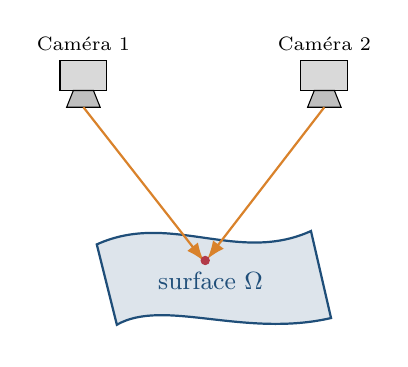
\begin{tikzpicture}[scale=0.85]
        \fill[pyblue!15] (-1.6,0) .. controls (-0.5,0.5) and (0.5,-0.3) .. (1.6,0.2)
          -- (1.9,-1.1) .. controls (0.6,-1.4) and (-0.6,-0.8) .. (-1.3,-1.2) -- cycle;
        \draw[pyblue,thick] (-1.6,0) .. controls (-0.5,0.5) and (0.5,-0.3) .. (1.6,0.2)
          -- (1.9,-1.1) .. controls (0.6,-1.4) and (-0.6,-0.8) .. (-1.3,-1.2) -- cycle;
        \node[pyblue] at (0.1,-0.55) {\small surface $\Omega$};
        \foreach \x/\n in {-1.8/1, 1.8/2}{
          \draw[fill=gray!30] (\x-0.35,2.3) rectangle (\x+0.35,2.75);
          \draw[fill=gray!50] (\x-0.15,2.3) -- (\x+0.15,2.3) -- (\x+0.25,2.05) -- (\x-0.25,2.05) -- cycle;
          \node at (\x,3.0) {\scriptsize Caméra \n};
        }
        \draw[-{Latex},pyorange,thick] (-1.8,2.05) -- (0.0,-0.25);
        \draw[-{Latex},pyorange,thick] (1.8,2.05) -- (0.05,-0.22);
        \fill[pyred] (0.02,-0.24) circle (2pt);
      \end{tikzpicture}
    \end{column}
  \end{columns}
\end{frame}
 
% ---------------------------------------------------------------------
\begin{frame}[fragile]{Dépendances et conventions}
  \begin{columns}[T]
    \begin{column}{0.50\textwidth}\small
      \textbf{Dépendances}
      \begin{itemize}
        \item obligatoires : \texttt{numpy}, \texttt{scipy}, \texttt{matplotlib},
              \texttt{cv2}, \texttt{pysolvegn} ;
        \item optionnelles, importées à l'usage : \texttt{open3d}, \texttt{pyvista},
              \texttt{meshio}, \texttt{h5py}\dots
      \end{itemize}
\begin{lstlisting}
mesh.cast_rays(rays)
# ImportError : cast_rays requires 'open3d'
#   pip install open3d
\end{lstlisting}
    \end{column}
    \begin{column}{0.46\textwidth}\small
      \textbf{Coordonnées image}
      \begin{itemize}
        \item $(x, y)$ = (colonne, ligne), $y$ vers le bas ;
        \item pixel $(u, v)$ = (ligne, colonne) ;
        \item centres des pixels aux entiers.
      \end{itemize}
      \medskip
      \centering
      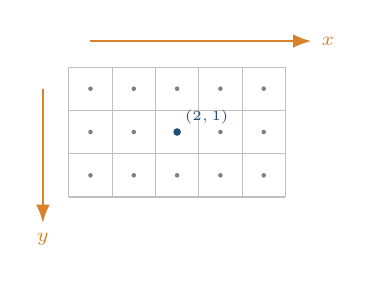
\begin{tikzpicture}[scale=0.55]
        \draw[step=1, gray!50] (0,0) grid (5,-3);
        \foreach \x in {0,...,4}{\foreach \y in {0,...,2}{\fill[gray] (\x+0.5,-\y-0.5) circle (1.5pt);}}
        \draw[->,thick,pyorange] (0.5,0.6) -- (5.6,0.6) node[right,font=\scriptsize]{$x$};
        \draw[->,thick,pyorange] (-0.6,-0.5) -- (-0.6,-3.6) node[below,font=\scriptsize]{$y$};
        \node[font=\tiny, pyblue] at (2.5,-1.5) [above right=-1pt] {$(2, 1)$};
        \fill[pyblue] (2.5,-1.5) circle (2.5pt);
      \end{tikzpicture}
    \end{column}
  \end{columns}
\end{frame}
 
% ---------------------------------------------------------------------
\begin{frame}{Organisation de \texttt{pysdic} : trois couches}
  \centering
  \resizebox{\linewidth}{!}{%
  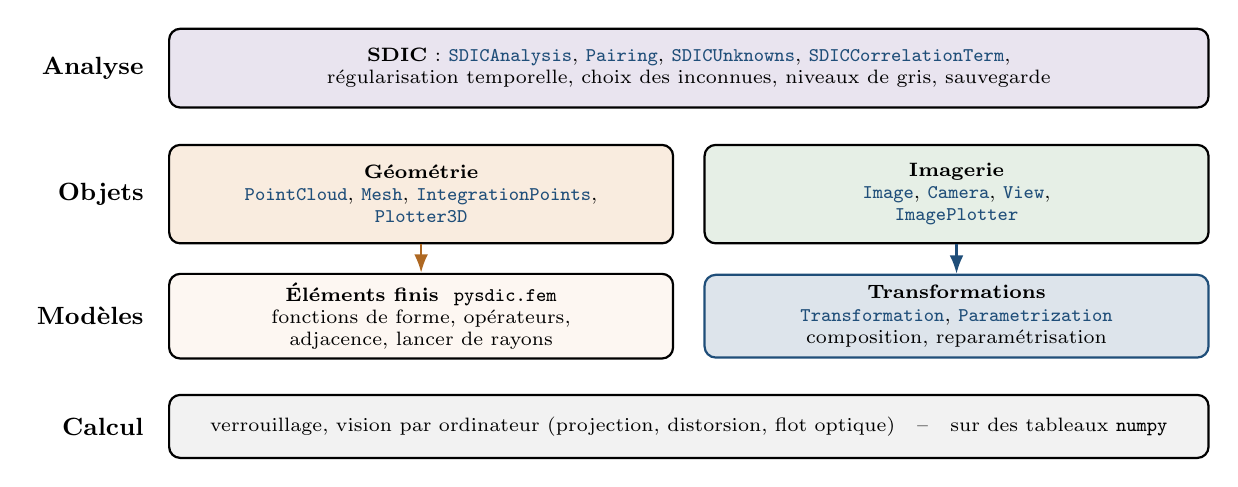
\begin{tikzpicture}[
      layer/.style={draw, rounded corners, thick, minimum height=1.0cm, align=center, font=\scriptsize},
      lab/.style={font=\small\bfseries, anchor=east}]
    \node[layer, fill=pypurple!15, minimum width=13.2cm] (analysis) at (0,2.95)
      {\textbf{SDIC} : \cls{SDICAnalysis}, \cls{Pairing}, \cls{SDICUnknowns}, \cls{SDICCorrelationTerm},\\
       régularisation temporelle, choix des inconnues, niveaux de gris, sauvegarde};
    \node[layer, fill=pyorange!15, minimum width=6.4cm, minimum height=1.25cm] (geo) at (-3.4,1.35)
      {\textbf{Géométrie}\\\cls{PointCloud}, \cls{Mesh}, \cls{IntegrationPoints},\\\cls{Plotter3D}};
    \node[layer, fill=pygreen!12, minimum width=6.4cm, minimum height=1.25cm] (img) at (3.4,1.35)
      {\textbf{Imagerie}\\\cls{Image}, \cls{Camera}, \cls{View},\\\cls{ImagePlotter}};
    \node[layer, fill=pyorange!6, minimum width=6.4cm, minimum height=1.05cm] (fem) at (-3.4,-0.2)
      {\textbf{Éléments finis} \ \texttt{pysdic.fem}\\fonctions de forme, opérateurs,\\adjacence, lancer de rayons};
    \node[layer, fill=pyblue!15, draw=pyblue, minimum width=6.4cm, minimum height=1.05cm] (tr) at (3.4,-0.2)
      {\textbf{Transformations}\\\cls{Transformation}, \cls{Parametrization}\\composition, reparamétrisation};
    \draw[->, thick, pyorange!80!black] (geo) -- (fem);
    \draw[->, thick, pyblue] (img) -- (tr);
    \node[layer, fill=gray!10, minimum width=13.2cm, minimum height=0.8cm] (calc) at (0,-1.6)
      {verrouillage, vision par ordinateur (projection, distorsion, flot optique)\quad --\quad sur des tableaux \texttt{numpy}};
    \node[lab] at (-6.8,2.95) {Analyse};
    \node[lab] at (-6.8,1.35) {Objets};
    \node[lab] at (-6.8,-0.2) {Modèles};
    \node[lab] at (-6.8,-1.6) {Calcul};
  \end{tikzpicture}}
\end{frame}
 
% ---------------------------------------------------------------------
\begin{frame}[fragile]{Partager et verrouiller}
  \begin{columns}[T]
    \begin{column}{0.48\textwidth}
      \textbf{Objets \textcolor{pyred}{partagés}}

      \smallskip
      \scriptsize Les objets ne sont \alert{jamais copiés} : deux caméras construites avec
      la même extrinsèque utilisent \alert{le même objet}.
\begin{lstlisting}
ext = PerspectiveExtrinsic(...)
cam_1 = Camera(..., extrinsic=ext, ...)
cam_2 = Camera(..., extrinsic=ext, ...)
 
cam_1.extrinsic.parameters = p
cam_2.extrinsic.parameters   # p aussi !
\end{lstlisting}
      \textcolor{pyred}{\textbf{Attention :}} modifier l'un modifie \alert{tous} ceux qui
      le partagent.
    \end{column}
    \begin{column}{0.50\textwidth}
      \textbf{Objets \textcolor{pyred}{verrouillés}}

      \smallskip
      \scriptsize Une analyse (\cls{SDICAnalysis}) a besoin d'un état \alert{invariant} : elle verrouille
      son maillage.
\begin{lstlisting}[basicstyle=\ttfamily\tiny]
mesh = Mesh(...)
mesh.is_locked          # False
 
analysis = SDICAnalysis(mesh, views)
mesh.is_locked          # True : verrouillé par l'analyse
 
mesh.coordinates = X
# RuntimeError: Cannot set the coordinates: this Mesh
#   is locked. It is used by an SDIC analysis, whose
#   operators [...] assume that its vertices and
#   elements never change. [...] To use a modified
#   mesh, work on a copy (mesh.copy()) and create a
#   new analysis with it (analysis.with_mesh(new_mesh)).
 
new_mesh = mesh.copy()  # déverrouillé
\end{lstlisting}
      Messages \alert{détaillés} : qui verrouille, pourquoi, et quoi faire.
    \end{column}
  \end{columns}
\end{frame}
 
% =====================================================================
\section{Géométrie}
% =====================================================================
 
\begin{frame}{Maillage et points d'intégration : ce qu'on définit}
  \centering
  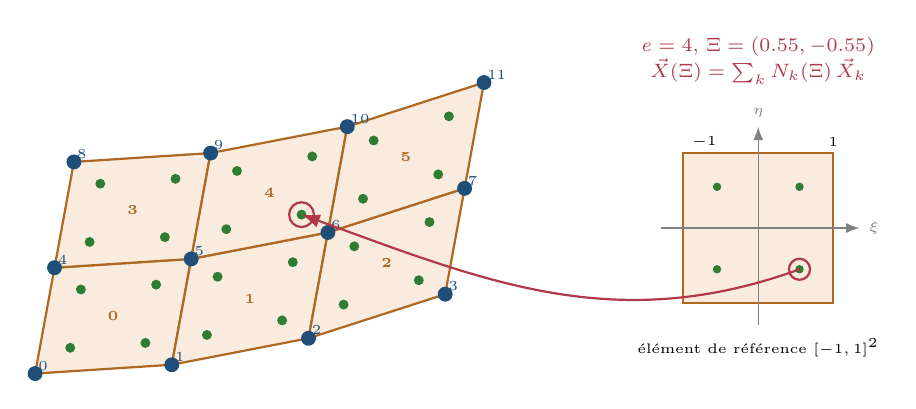
\begin{tikzpicture}[scale=1.12]
    \filldraw[fill=pyorange!15, draw=pyorange!80!black, thick] (0.000,0.000) -- (1.550,0.100) -- (1.770,1.300) -- (0.220,1.200) -- cycle;
    \node[font=\tiny\bfseries, text=pyorange!80!black] at (0.885,0.650) {0};
    \filldraw[fill=pyorange!15, draw=pyorange!80!black, thick] (1.550,0.100) -- (3.100,0.400) -- (3.320,1.600) -- (1.770,1.300) -- cycle;
    \node[font=\tiny\bfseries, text=pyorange!80!black] at (2.435,0.850) {1};
    \filldraw[fill=pyorange!15, draw=pyorange!80!black, thick] (3.100,0.400) -- (4.650,0.900) -- (4.870,2.100) -- (3.320,1.600) -- cycle;
    \node[font=\tiny\bfseries, text=pyorange!80!black] at (3.985,1.250) {2};
    \filldraw[fill=pyorange!15, draw=pyorange!80!black, thick] (0.220,1.200) -- (1.770,1.300) -- (1.990,2.500) -- (0.440,2.400) -- cycle;
    \node[font=\tiny\bfseries, text=pyorange!80!black] at (1.105,1.850) {3};
    \filldraw[fill=pyorange!15, draw=pyorange!80!black, thick] (1.770,1.300) -- (3.320,1.600) -- (3.540,2.800) -- (1.990,2.500) -- cycle;
    \node[font=\tiny\bfseries, text=pyorange!80!black] at (2.655,2.050) {4};
    \filldraw[fill=pyorange!15, draw=pyorange!80!black, thick] (3.320,1.600) -- (4.870,2.100) -- (5.090,3.300) -- (3.540,2.800) -- cycle;
    \node[font=\tiny\bfseries, text=pyorange!80!black] at (4.205,2.450) {5};
    \fill[pygreen] (0.398,0.292) circle (1.6pt);
    \fill[pygreen] (1.251,0.347) circle (1.6pt);
    \fill[pygreen] (1.372,1.008) circle (1.6pt);
    \fill[pygreen] (0.519,0.953) circle (1.6pt);
    \fill[pygreen] (1.948,0.438) circle (1.6pt);
    \fill[pygreen] (2.801,0.603) circle (1.6pt);
    \fill[pygreen] (2.922,1.263) circle (1.6pt);
    \fill[pygreen] (2.069,1.098) circle (1.6pt);
    \fill[pygreen] (3.498,0.782) circle (1.6pt);
    \fill[pygreen] (4.351,1.058) circle (1.6pt);
    \fill[pygreen] (4.472,1.718) circle (1.6pt);
    \fill[pygreen] (3.619,1.443) circle (1.6pt);
    \fill[pygreen] (0.618,1.492) circle (1.6pt);
    \fill[pygreen] (1.471,1.547) circle (1.6pt);
    \fill[pygreen] (1.592,2.208) circle (1.6pt);
    \fill[pygreen] (0.739,2.153) circle (1.6pt);
    \fill[pygreen] (2.168,1.637) circle (1.6pt);
    \fill[pygreen] (3.021,1.802) circle (1.6pt);
    \fill[pygreen] (3.142,2.462) circle (1.6pt);
    \fill[pygreen] (2.289,2.297) circle (1.6pt);
    \fill[pygreen] (3.718,1.982) circle (1.6pt);
    \fill[pygreen] (4.571,2.258) circle (1.6pt);
    \fill[pygreen] (4.692,2.917) circle (1.6pt);
    \fill[pygreen] (3.839,2.643) circle (1.6pt);
    \fill[pyblue] (0.000,0.000) circle (2.4pt);
    \node[font=\tiny, text=pyblue, anchor=south west, inner sep=1pt] at (0.000,0.000) {0};
    \fill[pyblue] (1.550,0.100) circle (2.4pt);
    \node[font=\tiny, text=pyblue, anchor=south west, inner sep=1pt] at (1.550,0.100) {1};
    \fill[pyblue] (3.100,0.400) circle (2.4pt);
    \node[font=\tiny, text=pyblue, anchor=south west, inner sep=1pt] at (3.100,0.400) {2};
    \fill[pyblue] (4.650,0.900) circle (2.4pt);
    \node[font=\tiny, text=pyblue, anchor=south west, inner sep=1pt] at (4.650,0.900) {3};
    \fill[pyblue] (0.220,1.200) circle (2.4pt);
    \node[font=\tiny, text=pyblue, anchor=south west, inner sep=1pt] at (0.220,1.200) {4};
    \fill[pyblue] (1.770,1.300) circle (2.4pt);
    \node[font=\tiny, text=pyblue, anchor=south west, inner sep=1pt] at (1.770,1.300) {5};
    \fill[pyblue] (3.320,1.600) circle (2.4pt);
    \node[font=\tiny, text=pyblue, anchor=south west, inner sep=1pt] at (3.320,1.600) {6};
    \fill[pyblue] (4.870,2.100) circle (2.4pt);
    \node[font=\tiny, text=pyblue, anchor=south west, inner sep=1pt] at (4.870,2.100) {7};
    \fill[pyblue] (0.440,2.400) circle (2.4pt);
    \node[font=\tiny, text=pyblue, anchor=south west, inner sep=1pt] at (0.440,2.400) {8};
    \fill[pyblue] (1.990,2.500) circle (2.4pt);
    \node[font=\tiny, text=pyblue, anchor=south west, inner sep=1pt] at (1.990,2.500) {9};
    \fill[pyblue] (3.540,2.800) circle (2.4pt);
    \node[font=\tiny, text=pyblue, anchor=south west, inner sep=1pt] at (3.540,2.800) {10};
    \fill[pyblue] (5.090,3.300) circle (2.4pt);
    \node[font=\tiny, text=pyblue, anchor=south west, inner sep=1pt] at (5.090,3.300) {11};
    \draw[pyred, thick] (3.021,1.802) circle (4pt);
    \coordinate (P) at (3.021,1.802);
    % Élément de référence
    \begin{scope}[shift={(8.2,1.65)}, scale=0.85]
      \filldraw[fill=pyorange!15, draw=pyorange!80!black, thick] (-1,-1) rectangle (1,1);
      \draw[->,gray] (-1.3,0) -- (1.35,0) node[right,font=\tiny]{$\xi$};
      \draw[->,gray] (0,-1.3) -- (0,1.35) node[above,font=\tiny]{$\eta$};
      \foreach \a/\b in {-0.55/-0.55, 0.55/-0.55, 0.55/0.55, -0.55/0.55}{\fill[pygreen] (\a,\b) circle (1.6pt);}
      \draw[pyred, thick] (0.55,-0.55) circle (4pt);
      \coordinate (Q) at (0.55,-0.55);
      \node[font=\tiny, below] at (0,-1.35) {élément de référence $[-1, 1]^2$};
      \node[font=\tiny] at (-0.72,1.15) {$-1$}; \node[font=\tiny] at (1.0,1.15) {$1$};
    \end{scope}
    \draw[->, thick, pyred] (Q) to[out=200, in=-20] (P);
    \node[font=\scriptsize, align=center, text=pyred] at (8.2,3.55)
      {$e = 4$, $\Xi = (0.55, -0.55)$\\$\vec{X}(\Xi) = \sum_k N_k(\Xi)\,\vec{X}_k$};
  \end{tikzpicture}
 
  \medskip
  \scriptsize
  \begin{tabular}{@{}r@{\quad}l@{}}
    \textbf{Maillage} &
    \textcolor{pyblue}{$\bullet$} sommets \texttt{mesh.vertices}
    \qquad \textcolor{pyorange}{$\blacksquare$} éléments \texttt{mesh.connectivity} \\
    \textbf{Points d'intégration} &
    \textcolor{pygreen}{$\bullet$} \texttt{IntegrationPoints} : $(e, \Xi, w)$ \\
  \end{tabular}
 
  \smallskip
  \small Un point d'intégration est repéré \alert{dans un élément}, pas dans l'espace :
  il suit les sommets quand le maillage se déforme.
\end{frame}
 
% ---------------------------------------------------------------------
\begin{frame}{Géométrie : comment les objets s'emboîtent}
  \centering
  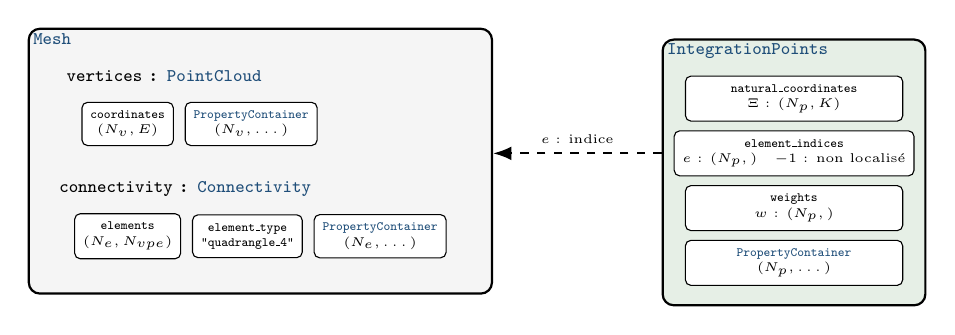
\begin{tikzpicture}[scale=0.92, every node/.append style={transform shape}]
    % PointCloud
    \node[attr] (coords) at (0,0) {\code{coordinates}\\$(N_v, E)$};
    \node[attr, right=0.15cm of coords] (pprops) {\cls{PropertyContainer}\\$(N_v, \dots)$};
    \begin{scope}[on background layer]
      \node[container, fill=pyblue!10, fit=(coords)(pprops), inner ysep=10pt, yshift=3pt] (pc) {};
    \end{scope}
    \node[ctitle] at (pc.north west) {\code{vertices} : \cls{PointCloud}};
    % Connectivity
    \node[attr] (elems) at (0,-1.55) {\code{elements}\\$(N_e, N_{vpe})$};
    \node[attr, right=0.15cm of elems] (etype) {\code{element\_type}\\\code{"quadrangle\_4"}};
    \node[attr, right=0.15cm of etype] (cprops) {\cls{PropertyContainer}\\$(N_e, \dots)$};
    \begin{scope}[on background layer]
      \node[container, fill=pyorange!10, fit=(elems)(cprops), inner ysep=10pt, yshift=3pt] (co) {};
    \end{scope}
    \node[ctitle] at (co.north west) {\code{connectivity} : \cls{Connectivity}};
    % Mesh
    \begin{scope}[on background layer]
      \node[container, fill=gray!8, fit=(pc)(co), inner sep=9pt, yshift=4pt] (mesh) {};
    \end{scope}
    \node[ctitle] at (mesh.north west) {\cls{Mesh}};
    % IntegrationPoints
    \node[attr, minimum width=3.0cm] (xi) at (9.2,0.35) {\code{natural\_coordinates}\\$\Xi$ : $(N_p, K)$};
    \node[attr, minimum width=3.0cm, below=0.12cm of xi] (ei) {\code{element\_indices}\\$e$ : $(N_p,)$\quad $-1$ : non localisé};
    \node[attr, minimum width=3.0cm, below=0.12cm of ei] (w) {\code{weights}\\$w$ : $(N_p,)$};
    \node[attr, minimum width=3.0cm, below=0.12cm of w] (iprops) {\cls{PropertyContainer}\\$(N_p, \dots)$};
    \begin{scope}[on background layer]
      \node[container, fill=pygreen!12, fit=(xi)(iprops), inner sep=8pt, inner ysep=10pt, yshift=3pt] (ip) {};
    \end{scope}
    \node[ctitle] at (ip.north west) {\cls{IntegrationPoints}};
    \draw[->,thick,dashed] (ip.west |- ei.west) -- node[above,font=\tiny]{$e$ : indice} (mesh.east |- ei.west);
  \end{tikzpicture}
 
  \medskip
  \begin{columns}[T]
    \begin{column}{0.44\textwidth}
      \centering\scriptsize
      \begin{tabular}{lcc}
        \toprule
        \code{element\_type} & $N_{vpe}$ & $K$ \\
        \midrule
        \code{segment\_2/3}    & 2 / 3 & 1 \\
        \code{triangle\_3/6}   & 3 / 6 & 2 \\
        \code{quadrangle\_4/8} & 4 / 8 & 2 \\
        \bottomrule
      \end{tabular}
    \end{column}
    \begin{column}{0.52\textwidth}\scriptsize
      Le type d'élément fixe le nombre de sommets par élément $N_{vpe}$, la dimension
      $K$ des coordonnées naturelles et les fonctions de forme :
      \[
        \vec{X}(\Xi) = \textstyle\sum_k N_k(\Xi)\, \vec{X}_k
      \]
    \end{column}
  \end{columns}
\end{frame}
 
% ---------------------------------------------------------------------
\begin{frame}[fragile]{\texttt{Mesh} dans le code}
  \begin{columns}[T]
    \begin{column}{0.52\textwidth}
\begin{lstlisting}
from pysdic import Mesh
 
# coords (N_v, 3), elements (N_e, 4)
coords = [[0, 0, 0], [1, 0, 0], [2, 0, 0],
          [0, 1, 0], [1, 1, 0], [2, 1, 0]]
elements = [[0, 1, 4, 3], [1, 2, 5, 4]]
mesh = Mesh(coords, elements,
            element_type="quadrangle_4")
 
mesh.vertices.coordinates   # (N_v, 3)
mesh.connectivity.elements  # (N_e, 4)
 
# Des propriétés sur les sommets et les éléments
mesh.vertices["temperature"] = T   # (N_v,)
mesh.connectivity["material"] = [0, 1]
\end{lstlisting}
    \end{column}
    \begin{column}{0.44\textwidth}
\begin{lstlisting}
mesh.to_vtk_file("surface.vtk")
mesh = Mesh.from_vtk_file("surface.vtk")
 
mesh.to_json_file("surface.json")
mesh = Mesh.from_json_file(
    "surface.json")
\end{lstlisting}
      \vspace{-4pt}
      \scriptsize Deux maillages peuvent partager les \alert{mêmes sommets} ou la
      \alert{même connectivité} :
\begin{lstlisting}[basicstyle=\ttfamily\tiny]
mesh_a = Mesh(pc, conn_a)
mesh_b = Mesh(pc, conn_b)  # mêmes sommets
mesh_b.vertices is mesh_a.vertices  # True
\end{lstlisting}
      \centering
      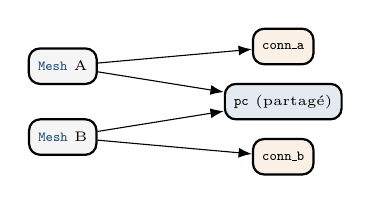
\begin{tikzpicture}[o/.style={draw, rounded corners, thick, font=\tiny, minimum height=0.45cm, align=center}]
        \node[o, fill=gray!8] (m1) at (0,0) {\cls{Mesh} A};
        \node[o, fill=gray!8] (m2) at (0,-0.9) {\cls{Mesh} B};
        \node[o, fill=pyorange!12] (c1) at (2.8,0.25) {\code{conn\_a}};
        \node[o, fill=pyblue!12] (v) at (2.8,-0.45) {\code{pc} (partagé)};
        \node[o, fill=pyorange!12] (c2) at (2.8,-1.15) {\code{conn\_b}};
        \draw[->] (m1) -- (v); \draw[->] (m2) -- (v);
        \draw[->] (m1) -- (c1); \draw[->] (m2) -- (c2);
      \end{tikzpicture}
    \end{column}
  \end{columns}
\end{frame}
 
% ---------------------------------------------------------------------
\begin{frame}[fragile]{\texttt{IntegrationPoints} : deux façons de les créer}
  \begin{columns}[T]
    \begin{column}{0.48\textwidth}
      \textbf{Par coordonnées}
\begin{lstlisting}
from pysdic import IntegrationPoints
 
ip = IntegrationPoints(
    natural_coordinates=xi_p,  # Xi (N_p, K)
    element_indices=e_p,       # e  (N_p,)
    weights=w_p)               # w  (N_p,)
\end{lstlisting}
      \scriptsize $\Xi$ : position dans l'élément de référence ; $e$ : élément qui
      contient le point ; $w$ : poids.
    \end{column}
    \begin{column}{0.48\textwidth}
      \textbf{Par lancer de rayons} \scriptsize(un point par pixel)
\begin{lstlisting}
rays = camera.get_camera_rays()  # (H, W, 6)
ip = mesh.cast_rays(rays)        # H*W points
ip.is_located()                  # e != -1
ip = ip.remove_unlocated()
\end{lstlisting}
    \end{column}
  \end{columns}
\end{frame}
 
% ---------------------------------------------------------------------
\begin{frame}[fragile]{Maillage $\times$ points d'intégration}
  \centering
  \resizebox{\linewidth}{!}{%
  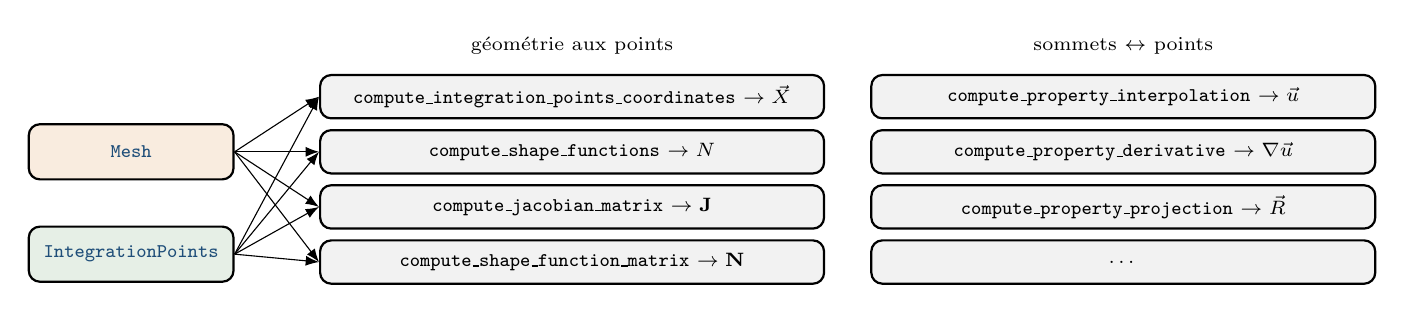
\begin{tikzpicture}[op/.style={box, fill=gray!10, minimum width=6.4cm, minimum height=0.55cm}]
    \node[box, fill=pyorange!15, minimum width=2.6cm] (m) at (0,0.2) {\cls{Mesh}};
    \node[box, fill=pygreen!12, minimum width=2.6cm] (i) at (0,-1.1) {\cls{IntegrationPoints}};
    \node[op] (o1) at (5.6,0.9)   {\code{compute\_integration\_points\_coordinates} $\to \vec{X}$};
    \node[op] (o2) at (5.6,0.2)   {\code{compute\_shape\_functions} $\to N$};
    \node[op] (o3) at (5.6,-0.5)  {\code{compute\_jacobian\_matrix} $\to \mathbf{J}$};
    \node[op] (o4) at (5.6,-1.2)  {\code{compute\_shape\_function\_matrix} $\to \mathbf{N}$};
    \node[op] (o5) at (12.6,0.9)  {\code{compute\_property\_interpolation} $\to \vec{u}$};
    \node[op] (o6) at (12.6,0.2)  {\code{compute\_property\_derivative} $\to \nabla\vec{u}$};
    \node[op] (o7) at (12.6,-0.5) {\code{compute\_property\_projection} $\to \vec{R}$};
    \node[op] (o8) at (12.6,-1.2) {\dots};
    \foreach \t in {o1,o2,o3,o4}{\draw[->] (m.east) -- (\t.west); \draw[->] (i.east) -- (\t.west);}
    \node[font=\scriptsize] at (5.6,1.55) {géométrie aux points};
    \node[font=\scriptsize] at (12.6,1.55) {sommets $\leftrightarrow$ points};
  \end{tikzpicture}}
 
  \medskip
\begin{lstlisting}[basicstyle=\ttfamily\scriptsize]
X = mesh.compute_integration_points_coordinates(ip)  # (N_p, E)       positions
N = mesh.compute_shape_functions(ip)                 # (N_p, N_vpe)   N_k aux points
J = mesh.compute_jacobian_matrix(ip)                 # (N_p, E, K)    dX / dXi
N_mat = mesh.compute_shape_function_matrix(ip, sparse=True)  # (N_p, N_v)
u = mesh.compute_property_interpolation(U, ip)       # (N_p, 3)       sommets -> points
grad_u = mesh.compute_property_derivative(U, ip)     # (N_p, 3, 3)
R = mesh.compute_property_projection(r, ip)          # (N_v, ...)     points -> sommets
\end{lstlisting}
\end{frame}
 
% ---------------------------------------------------------------------
\begin{frame}[fragile]{Visualisation : \texttt{Plotter3D}}
  \begin{columns}[T]
    \begin{column}{0.42\textwidth}
      Basé sur PyVista :
      \begin{itemize}\small
        \item \code{add\_mesh} : faces, arêtes, sommets, propriétés,
              texture (UV map), \code{warp\_by} ;
        \item \code{add\_point\_cloud} ;
        \item \code{add\_integration\_points} : positions dans le maillage
              (déformé) ;
        \item champs de vecteurs (flèches).
      \end{itemize}
      \medskip
      \small \code{warp\_by} : un tableau $(N_v, E)$ ou le nom d'une propriété
      des sommets.
    \end{column}
    \begin{column}{0.56\textwidth}
\begin{lstlisting}
from pysdic import Plotter3D
 
plotter = Plotter3D()
plotter.add_mesh(
    mesh,
    warp_by=displacement,
    vertex_property=displacement,
    show_bar=True,
)
plotter.add_integration_points(
    ip, mesh, warp_by=displacement,
    color="red", size=4,
)
plotter.show()
\end{lstlisting}
    \end{column}
  \end{columns}
\end{frame}
 
 
% =====================================================================
\section{Imagerie}
% =====================================================================
 
% ---------------------------------------------------------------------
\begin{frame}{Imagerie : ce qu'on définit}
  \centering
  \resizebox{\linewidth}{!}{%
  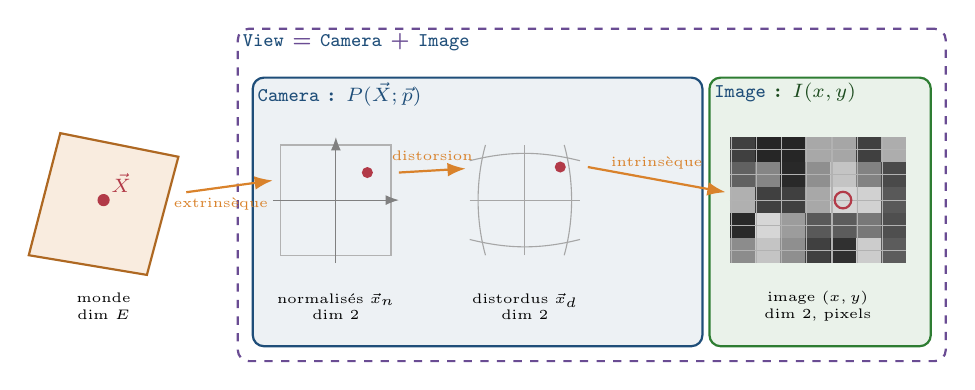
\begin{tikzpicture}
    % Monde
    \filldraw[fill=pyorange!15, draw=pyorange!80!black, thick]
      (-0.6,-0.7) -- (0.9,-0.95) -- (1.3,0.55) -- (-0.2,0.85) -- cycle;
    \fill[pyred] (0.35,0.0) circle (2.2pt) node[above right=-1pt, font=\scriptsize]{$\vec{X}$};
    \node[font=\tiny, align=center] at (0.35,-1.35) {monde\\dim $E$};
    % Normalisés
    \draw[gray!60] (2.6,-0.7) rectangle (4.0,0.7);
    \draw[->,gray] (2.5,0) -- (4.1,0); \draw[->,gray] (3.3,-0.8) -- (3.3,0.8);
    \fill[pyred] (3.7,0.35) circle (2pt);
    \node[font=\tiny, align=center] at (3.3,-1.35) {normalisés $\vec{x}_n$\\dim 2};
    % Distordus
    \foreach \t in {-0.5,0,0.5}{
      \draw[gray!70] (5.0,\t) .. controls (5.5,\t*1.25) and (5.9,\t*1.25) .. (6.4,\t);
      \draw[gray!70] (5.7+\t,-0.7) .. controls (5.7+\t*1.25,-0.25) and (5.7+\t*1.25,0.25) .. (5.7+\t,0.7);}
    \fill[pyred] (6.15,0.42) circle (2pt);
    \node[font=\tiny, align=center] at (5.7,-1.35) {distordus $\vec{x}_d$\\dim 2};
    % Image (pixels)
    \fill[black!45] (8.30,-0.80) rectangle ++(0.32,0.32);
    \fill[black!84] (8.30,-0.48) rectangle ++(0.32,0.32);
    \fill[black!31] (8.30,-0.16) rectangle ++(0.32,0.32);
    \fill[black!62] (8.30,0.16) rectangle ++(0.32,0.32);
    \fill[black!75] (8.30,0.48) rectangle ++(0.32,0.32);
    \fill[black!23] (8.62,-0.80) rectangle ++(0.32,0.32);
    \fill[black!16] (8.62,-0.48) rectangle ++(0.32,0.32);
    \fill[black!75] (8.62,-0.16) rectangle ++(0.32,0.32);
    \fill[black!48] (8.62,0.16) rectangle ++(0.32,0.32);
    \fill[black!85] (8.62,0.48) rectangle ++(0.32,0.32);
    \fill[black!44] (8.94,-0.80) rectangle ++(0.32,0.32);
    \fill[black!39] (8.94,-0.48) rectangle ++(0.32,0.32);
    \fill[black!75] (8.94,-0.16) rectangle ++(0.32,0.32);
    \fill[black!84] (8.94,0.16) rectangle ++(0.32,0.32);
    \fill[black!85] (8.94,0.48) rectangle ++(0.32,0.32);
    \fill[black!75] (9.26,-0.80) rectangle ++(0.32,0.32);
    \fill[black!65] (9.26,-0.48) rectangle ++(0.32,0.32);
    \fill[black!34] (9.26,-0.16) rectangle ++(0.32,0.32);
    \fill[black!44] (9.26,0.16) rectangle ++(0.32,0.32);
    \fill[black!34] (9.26,0.48) rectangle ++(0.32,0.32);
    \fill[black!81] (9.58,-0.80) rectangle ++(0.32,0.32);
    \fill[black!64] (9.58,-0.48) rectangle ++(0.32,0.32);
    \fill[black!16] (9.58,-0.16) rectangle ++(0.32,0.32);
    \fill[black!23] (9.58,0.16) rectangle ++(0.32,0.32);
    \fill[black!35] (9.58,0.48) rectangle ++(0.32,0.32);
    \fill[black!20] (9.90,-0.80) rectangle ++(0.32,0.32);
    \fill[black!53] (9.90,-0.48) rectangle ++(0.32,0.32);
    \fill[black!18] (9.90,-0.16) rectangle ++(0.32,0.32);
    \fill[black!49] (9.90,0.16) rectangle ++(0.32,0.32);
    \fill[black!75] (9.90,0.48) rectangle ++(0.32,0.32);
    \fill[black!64] (10.22,-0.80) rectangle ++(0.32,0.32);
    \fill[black!69] (10.22,-0.48) rectangle ++(0.32,0.32);
    \fill[black!65] (10.22,-0.16) rectangle ++(0.32,0.32);
    \fill[black!71] (10.22,0.16) rectangle ++(0.32,0.32);
    \fill[black!32] (10.22,0.48) rectangle ++(0.32,0.32);
    \draw[gray!60, step=0.32] (8.3,-0.8) grid (10.54,0.80);
    \draw[pyred, thick] (9.74,0.00) circle (3pt);
    \node[font=\tiny, align=center] at (9.42,-1.35) {image $(x, y)$\\dim 2, pixels};
    % Flèches
    \draw[->,thick,pyorange] (1.4,0.1) -- node[below,font=\tiny,pos=0.4]{extrinsèque} (2.5,0.25);
    \draw[->,thick,pyorange] (4.1,0.35) -- node[above,font=\tiny]{distorsion} (4.95,0.4);
    \draw[->,thick,pyorange] (6.5,0.42) -- node[above,font=\tiny]{intrinsèque} (8.25,0.1);
    % Conteneurs
    \begin{scope}[on background layer]
      \node[container, fill=pyblue!8, draw=pyblue, inner sep=3pt, fit={(2.35,-1.75) (7.85,1.45)}] (cam) {};
      \node[container, fill=pygreen!10, draw=pygreen, inner sep=3pt, fit={(8.15,-1.75) (10.75,1.45)}] (img) {};
      \node[container, dashed, draw=pypurple, inner sep=5pt, fit={(cam.south west) (img.north east) (2.3,2.0)}] (view) {};
    \end{scope}
    \node[ctitle, text=pyblue] at (cam.north west) {\cls{Camera} : $P(\vec{X}; \vec{p})$};
    \node[ctitle, text=pygreen!60!black] at (img.north west) {\cls{Image} : $I(x, y)$};
    \node[ctitle, text=pypurple] at (view.north west) {\cls{View} = \cls{Camera} + \cls{Image}};
  \end{tikzpicture}}
 
  \bigskip
  \[
    g = I\bigl(P(\vec{X}; \vec{p})\bigr)
    \qquad \text{niveau de gris du point matériel } \vec{X} \text{ vu par la vue}
  \]
  \small Les dérivées par rapport à $\vec{X}$ (\alert{mesure}) et à $\vec{p}$
  (\alert{étalonnage}) sont fournies.
\end{frame}
 
\begin{frame}{Imagerie : comment les objets s'emboîtent}
  \centering
  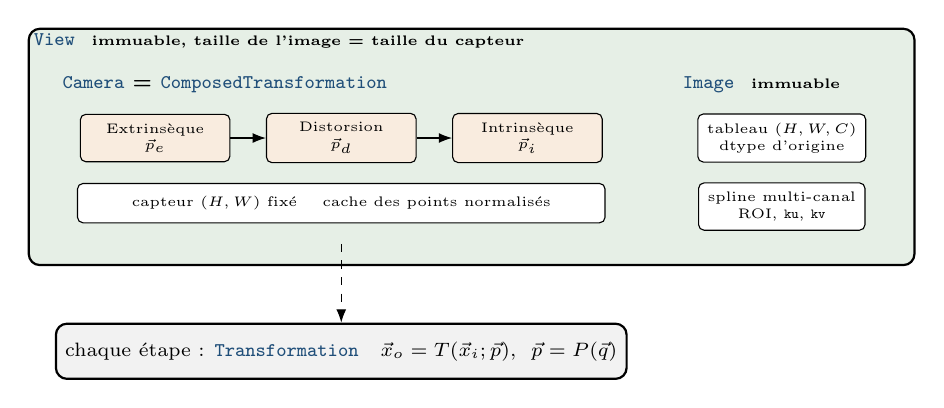
\begin{tikzpicture}
    % Transformations dans la Camera
    \node[attr, fill=pyorange!15, minimum width=1.9cm] (ex) at (0,0) {Extrinsèque\\$\vec{p}_e$};
    \node[attr, fill=pyorange!15, minimum width=1.9cm, right=0.45cm of ex] (di) {Distorsion\\$\vec{p}_d$};
    \node[attr, fill=pyorange!15, minimum width=1.9cm, right=0.45cm of di] (in) {Intrinsèque\\$\vec{p}_i$};
    \draw[->] (ex) -- (di); \draw[->] (di) -- (in);
    \node[attr, below=0.25cm of di, minimum width=6.7cm] (sensor) {capteur $(H, W)$ fixé \quad cache des points normalisés};
    \begin{scope}[on background layer]
      \node[container, fill=pyblue!10, fit=(ex)(in)(sensor), inner ysep=11pt, yshift=4pt] (cam) {};
    \end{scope}
    \node[ctitle] at (cam.north west) {\cls{Camera} = \cls{ComposedTransformation}};
    % Image
    \node[attr, right=1.2cm of in, yshift=0cm] (arr) {tableau $(H, W, C)$\\dtype d'origine};
    \node[attr, below=0.25cm of arr] (spl) {spline multi-canal\\ROI, \code{ku}, \code{kv}};
    \begin{scope}[on background layer]
      \node[container, fill=pyblue!10, fit=(arr)(spl), inner ysep=11pt, yshift=4pt] (im) {};
    \end{scope}
    \node[ctitle] at (im.north west) {\cls{Image}\ \ \tiny immuable};
    % View
    \begin{scope}[on background layer]
      \node[container, fill=pygreen!12, fit=(cam)(im), inner sep=10pt, yshift=5pt] (view) {};
    \end{scope}
    \node[ctitle] at (view.north west) {\cls{View}\ \ \tiny immuable, taille de l'image = taille du capteur};
    % Transformation générique
    \node[box, fill=gray!10, below=1.0cm of cam, minimum width=6.5cm] (tr)
      {chaque étape : \cls{Transformation}\quad $\vec{x}_o = T(\vec{x}_i; \vec{p})$,\ \ $\vec{p} = P(\vec{q})$};
    \draw[->,dashed] (cam.south) -- (tr.north);
  \end{tikzpicture}
 
  \medskip
  \small La nomenclature \cls{View} / \cls{Camera} / \cls{Image} reprend celle de
  \alert{uCheckmate} (H.~Matar, 2025). Les \cls{Transformation} et \cls{Parametrization}
  sont propres à \texttt{pysdic}. Transformations et capteur sont fixes : seuls les
  \alert{paramètres} changent.
\end{frame}
 
% ---------------------------------------------------------------------
\begin{frame}[fragile]{\texttt{Transformation} : $\vec{x}_o = T(\vec{x}_i ; \vec{p})$}
  \begin{columns}[T]
    \begin{column}{0.50\textwidth}\small
      Classe abstraite d'une application paramétrée
      $\mathbb{R}^{n_i} \to \mathbb{R}^{n_o}$, point par point :
      \begin{itemize}
        \item \code{apply} : $\vec{x}_o$, $\ \mathbf{J}_x = \partial T / \partial \vec{x}_i$,
              $\ \mathbf{J}_p = \partial T / \partial \vec{p}$ ;
        \item \code{invert} : $T^{-1}$ et ses jacobiennes ;
        \item \alert{paramètres} (dérivables, optimisés) vs \alert{constantes} ;
        \item \code{has\_apply\_dx}, \code{has\_apply\_dp}\dots : indiquent si une
              quantité est définie ;
        \item \alert{verrouillable} : une transformation verrouillée refuse
              \code{set\_parameters}.
      \end{itemize}
    \end{column}
    \begin{column}{0.48\textwidth}
\begin{lstlisting}
res = T.apply(x, dx=True, dp=True)
res.x            # (..., n_o)
res.jacobian_dx  # (..., n_o, n_i)
res.jacobian_dp  # (..., n_o, n_p)
 
T.parameters = p
T.to_json_file("extrinsic.json")
\end{lstlisting}
    \end{column}
  \end{columns}
\end{frame}
 
% ---------------------------------------------------------------------
\begin{frame}{Les modèles implémentés}
  \centering
  \renewcommand{\arraystretch}{1.05}
  \resizebox{\linewidth}{!}{%
  \begin{tabular}{@{}lll@{}}
    \toprule
    modèle & dim. & en une ligne \\
    \midrule
    \multicolumn{3}{@{}l}{\textbf{Extrinsèques} \quad monde $\to$ normalisés} \\
    \cls{NoExtrinsic} & 3D/2D $\to$ 2D & identité ; en 3D, $z$ ignoré (orthographique) \\
    \cls{PerspectiveExtrinsic} & 3D $\to$ 2D & pose $[R|T]$ puis division par $Z_c$ (OpenCV) \\
    \cls{OrthographicExtrinsic} & 3D $\to$ 2D & pose $[R|T]$ sans division par $Z_c$ \\
    \cls{WorldPlanePerspectiveExtrinsic} & 2D $\to$ 2D & perspective 3D sur le plan $Z_w = 0$ : $H = [\vec{r}_1, \vec{r}_2, T]$ \\
    \cls{WorldPlaneOrthographicExtrinsic} & 2D $\to$ 2D & orthographique 3D sur le plan $Z_w = 0$ (affine) \\
    \cls{PlanarRigidExtrinsic} & 2D $\to$ 2D & rigide plane : $\theta$ et $\vec{t}$ (3 paramètres) \\
    \cls{PlanarHomographicExtrinsic} & 2D $\to$ 2D & homographie plane $H$ (8 paramètres, $H_{22} = 1$) \\
    \midrule
    \multicolumn{3}{@{}l}{\textbf{Distorsions} \quad normalisés $\to$ distordus \quad (inverse par Newton)} \\
    \cls{NoDistortion} & 2D $\to$ 2D & identité \\
    \cls{BrownDistortion} & 2D $\to$ 2D & Brown--Conrady d'OpenCV (0, 4, 5, 8, 12 ou 14 paramètres) \\
    \cls{ZernikeDistortion} & 2D $\to$ 2D & déplacement sur les polynômes de Zernike, sur une ellipse \\
    \midrule
    \multicolumn{3}{@{}l}{\textbf{Intrinsèques} \quad distordus $\to$ image (pixels)} \\
    \cls{NoIntrinsic} & 2D $\to$ 2D & identité \\
    \cls{PinholeIntrinsic} & 2D $\to$ 2D & matrice $K$ : $f_x, f_y, c_x, c_y$, biais $s$ optionnel \\
    \bottomrule
  \end{tabular}}
\end{frame}
 
% ---------------------------------------------------------------------
\begin{frame}{Composition et reparamétrisation}
  \begin{columns}[T]
    \begin{column}{0.49\textwidth}
      \textbf{Composition} \hfill \code{T2 @ T1}
      \[
        T(\vec{x};\vec{p}) = T_2\bigl(T_1(\vec{x};\vec{p}_1);\vec{p}_2\bigr),
        \quad \vec{p} = [\vec{p}_1, \vec{p}_2]
      \]
      \[
        \mathbf{J}_p = \Bigl[\ \tfrac{\partial T_2}{\partial \vec{x}}\,\tfrac{\partial T_1}{\partial \vec{p}_1}
        \ \ \Big|\ \ \tfrac{\partial T_2}{\partial \vec{p}_2}\ \Bigr]
      \]
      \small Les transformations ne sont pas copiées : modifier $\vec{p}$ de la
      composition modifie chaque étape. Le verrou se propage aux étapes.
    \end{column}
    \begin{column}{0.49\textwidth}
      \textbf{Reparamétrisation} \hfill \cls{ReparametrizedTransformation}
      \[
        \tilde{T}(\vec{x};\vec{q}) = T\bigl(\vec{x}; P(\vec{q})\bigr)
      \]
      \[
        \mathbf{J}_q = \frac{\partial T}{\partial \vec{p}} \cdot \frac{\partial P}{\partial \vec{q}}
      \]
      \small Une \cls{Parametrization} $P$ change la \alert{modélisation} de la
      caméra : sous-ensemble de paramètres, modes PCA, etc.
    \end{column}
  \end{columns}
\end{frame}
 
% ---------------------------------------------------------------------
\begin{frame}[fragile]{\texttt{Camera} : projection et jacobiennes}
  \centering
  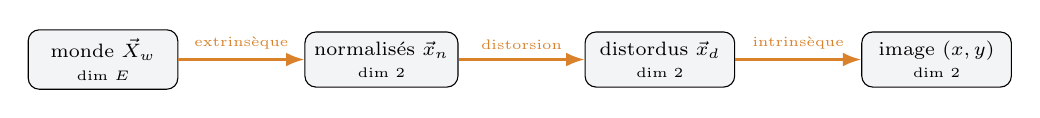
\begin{tikzpicture}[
      pt/.style={draw, rounded corners, fill=pygray, minimum width=1.9cm, minimum height=0.7cm, align=center, font=\scriptsize}]
    \node[pt] (w) {monde $\vec{X}_w$\\\tiny dim $E$};
    \node[pt, right=1.6cm of w] (n) {normalisés $\vec{x}_n$\\\tiny dim 2};
    \node[pt, right=1.6cm of n] (d) {distordus $\vec{x}_d$\\\tiny dim 2};
    \node[pt, right=1.6cm of d] (i) {image $(x, y)$\\\tiny dim 2};
    \draw[->,thick,pyorange] (w) -- node[above,font=\tiny]{extrinsèque} (n);
    \draw[->,thick,pyorange] (n) -- node[above,font=\tiny]{distorsion} (d);
    \draw[->,thick,pyorange] (d) -- node[above,font=\tiny]{intrinsèque} (i);
  \end{tikzpicture}
 
  \begin{columns}[T]
    \begin{column}{0.56\textwidth}
\begin{lstlisting}
from pysdic import (Camera, BrownDistortion,
    PerspectiveExtrinsic, PinholeIntrinsic)
 
camera = Camera(
    sensor_height=480, sensor_width=640,  # pixels
    extrinsic=PerspectiveExtrinsic.from_rt(
        rvec=[0.1, 0.2, 0.3], tvec=[12, 34, 56]),
    distortion=BrownDistortion(dist),
    intrinsic=PinholeIntrinsic.from_matrix(K))
 
res = camera.project(X, dx=True, dextrinsic=True)
res.image_points         # (..., 2)
res.jacobian_dx          # (..., 2, 3)
res.jacobian_dextrinsic  # (..., 2, N_e)
\end{lstlisting}
    \end{column}
    \begin{column}{0.42\textwidth}\small
      \begin{itemize}
        \item $\mathbf{J}_x$ : sensibilité au \alert{déplacement} ;
        \item $\mathbf{J}_p$ par blocs, paramètres $[\vec{p}_e, \vec{p}_d, \vec{p}_i]$ :
              \alert{étalonnage} ; les blocs non demandés valent NaN ;
        \item accepte aussi un \cls{PointCloud} ou un \cls{Mesh}.
      \end{itemize}
    \end{column}
  \end{columns}
\end{frame}
 
% ---------------------------------------------------------------------
\begin{frame}[fragile]{\texttt{Image} : niveaux de gris continus}
  \begin{columns}[T]
    \begin{column}{0.48\textwidth}\small
      \begin{itemize}
        \item tableau $(H, W)$ ou $(H, W, C)$, entier ou flottant, \code{dtype}
              d'origine conservé ;
        \item une spline \alert{multi-canal}, degrés \code{ku}, \code{kv}
              $\in [1, 5]$ (\texttt{scipy}) ;
        \item \code{roi} $=(x, y, w, h)$ : la vraie taille en pixels de la zone
              interpolée ;
        \item hors ROI : NaN ;
        \item valeurs et dérivées en \alert{un seul passage} ;
        \item \alert{immuable} : données copiées en lecture seule, aucun setter ;
              \code{with\_settings} rend une nouvelle image qui \alert{partage} les
              données.
      \end{itemize}
    \end{column}
    \begin{column}{0.50\textwidth}
\begin{lstlisting}
from pysdic import Image
 
image = Image.from_file(
    "ref.tif", roi=(100, 50, 400, 300))
image = Image.from_array(array)
 
# ordres (x, y) -> un tuple
I, Ix, Iy = image.evaluate_at_image_points(
    xy, derivatives=((0, 0), (1, 0), (0, 1)))
(I,) = image.evaluate_at_image_points(xy)
(I,) = image.evaluate_at_pixel_points(uv)
 
zoom = image.with_settings(
    roi=(0, 0, 200, 200), ku=5)
 
image.to_file("copy.png")     # dtype conservé
image.to_npz_file("ref.npz")  # + ROI, ku, kv
\end{lstlisting}
    \end{column}
  \end{columns}
\end{frame}
 
% ---------------------------------------------------------------------
\begin{frame}{\texttt{View} : partager caméras et images}
  \centering
  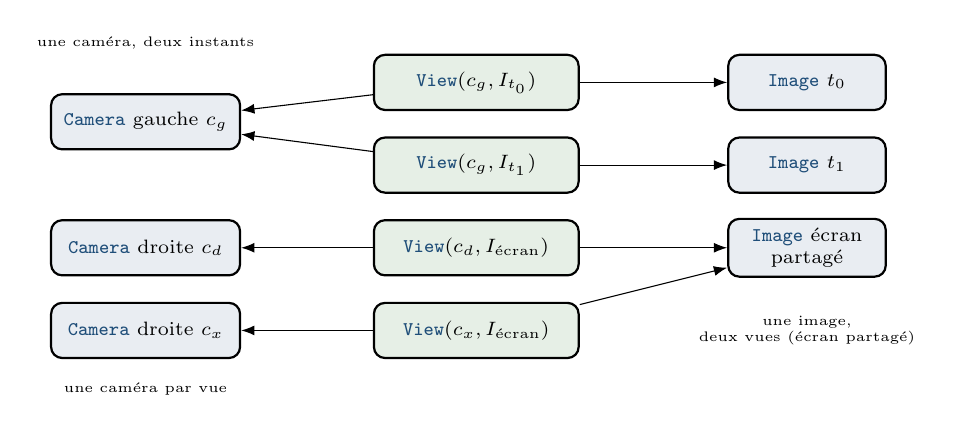
\begin{tikzpicture}
    \node[box, fill=pyblue!10, minimum width=2.4cm] (c1) at (0,0) {\cls{Camera} gauche $c_g$};
    \node[box, fill=pyblue!10, minimum width=2.4cm] (c2) at (0,-1.6) {\cls{Camera} droite $c_d$};
    \node[box, fill=pyblue!10, minimum width=2.4cm] (c3) at (0,-2.65) {\cls{Camera} droite $c_x$};
    \node[box, fill=pyblue!10, minimum width=2.0cm] (i0) at (8.4,0.5) {\cls{Image} $t_0$};
    \node[box, fill=pyblue!10, minimum width=2.0cm] (i1) at (8.4,-0.55) {\cls{Image} $t_1$};
    \node[box, fill=pyblue!10, minimum width=2.0cm] (i2) at (8.4,-1.6) {\cls{Image} écran\\partagé};
    \node[box, fill=pygreen!12, minimum width=2.6cm] (v0) at (4.2,0.5) {\cls{View}$(c_g, I_{t_0})$};
    \node[box, fill=pygreen!12, minimum width=2.6cm] (v1) at (4.2,-0.55) {\cls{View}$(c_g, I_{t_1})$};
    \node[box, fill=pygreen!12, minimum width=2.6cm] (v2) at (4.2,-1.6) {\cls{View}$(c_d, I_{\text{écran}})$};
    \node[box, fill=pygreen!12, minimum width=2.6cm] (v3) at (4.2,-2.65) {\cls{View}$(c_x, I_{\text{écran}})$};
    \draw[->] (v0) -- (c1); \draw[->] (v1) -- (c1); \draw[->] (v2) -- (c2); \draw[->] (v3) -- (c3);
    \draw[->] (v0) -- (i0); \draw[->] (v1) -- (i1); \draw[->] (v2) -- (i2); \draw[->] (v3) -- (i2);
    \node[font=\tiny, align=center] at (0,1.0) {une caméra, deux instants};
    \node[font=\tiny, align=center] at (0,-3.4) {une caméra par vue};
    \node[font=\tiny, align=center] at (8.4,-2.65) {une image,\\deux vues (écran partagé)};
  \end{tikzpicture}
 
  \medskip
  \[
    g = I\bigl(P(\vec{X})\bigr), \qquad
    \nabla_{\gamma}\bigl[I \circ P\bigr] = \nabla_x I\bigl(P(\vec{X})\bigr)\cdot\nabla_{\gamma} P(\vec{X}),
    \quad \gamma \in \{\vec{X}, \vec{p}\}
  \]
\end{frame}
 
% ---------------------------------------------------------------------
\begin{frame}[fragile]{\texttt{View} dans le code}
  \begin{columns}[T]
    \begin{column}{0.55\textwidth}
\begin{lstlisting}
from pysdic import View
 
view = View(camera, image)
res = view.image_project(X, dx=True,
                         dextrinsic=True)
res.gray_levels           # (..., C)
res.image_points          # (..., 2)
res.jacobian_dx           # (..., C, E)
res.jacobian_dextrinsic   # (..., C, N_e)
 
view.quick_visualize(mesh)
\end{lstlisting}
    \end{column}
    \begin{column}{0.43\textwidth}\small
      \begin{itemize}
        \item \cls{View} \alert{immuable} ;
        \item $C$ canaux par point ;
        \item hors ROI : NaN.
      \end{itemize}
      \medskip
      \code{jacobian\_dx} est exactement le gradient attendu par
      \code{assemble\_displacement\_}\allowbreak\code{jacobian\_matrix}.
    \end{column}
  \end{columns}
\end{frame}
 
% ---------------------------------------------------------------------
\begin{frame}[fragile]{Maillage $\times$ caméra}
  \centering
  \resizebox{0.95\linewidth}{!}{%
  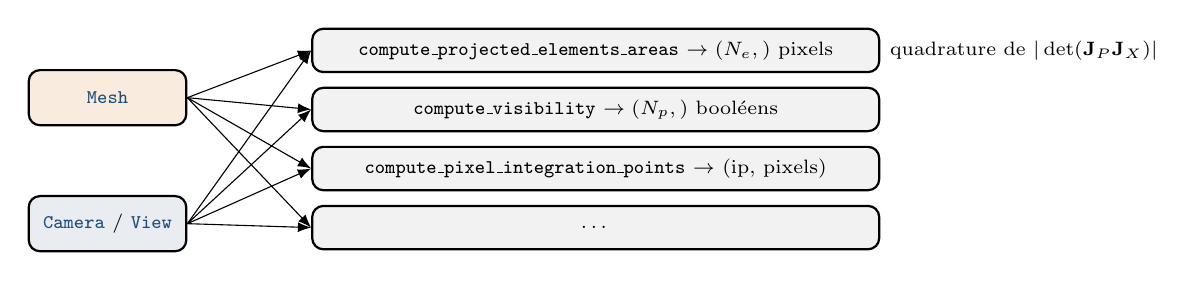
\begin{tikzpicture}[op/.style={box, fill=gray!10, minimum width=7.2cm, minimum height=0.55cm}]
    \node[box, fill=pyorange!15, minimum width=2.0cm] (m) at (0,0.3) {\cls{Mesh}};
    \node[box, fill=pyblue!10, minimum width=2.0cm] (c) at (0,-1.3) {\cls{Camera} / \cls{View}};
    \node[op] (a) at (6.2,0.9)   {\code{compute\_projected\_elements\_areas} $\to (N_e,)$ pixels};
    \node[op] (v) at (6.2,0.15)  {\code{compute\_visibility} $\to (N_p,)$ booléens};
    \node[op] (p) at (6.2,-0.6)  {\code{compute\_pixel\_integration\_points} $\to$ (ip, pixels)};
    \node[op] (d) at (6.2,-1.35) {\dots};
    \foreach \t in {a,v,p,d}{\draw[->] (m.east) -- (\t.west); \draw[->] (c.east) -- (\t.west);}
    \node[font=\scriptsize, anchor=west] at (a.east) {quadrature de $|\det(\mathbf{J}_P \mathbf{J}_X)|$};
  \end{tikzpicture}}
 
  \medskip
\begin{lstlisting}
from pysdic import (compute_projected_elements_areas, compute_visibility,
                    compute_pixel_integration_points)
 
areas = compute_projected_elements_areas(mesh, camera)
seen = compute_visibility(mesh, ip, view, warp_by=displacement)
ip_px, pixels = compute_pixel_integration_points(mesh, view)
\end{lstlisting}
\end{frame}
 
% ---------------------------------------------------------------------
\begin{frame}[fragile]{Visualisation : \texttt{ImagePlotter}}
  \begin{columns}[T]
    \begin{column}{0.42\textwidth}
      Basé sur \texttt{matplotlib}, dans le \alert{repère image} :
      \begin{itemize}\small
        \item source : une \cls{Camera}, une \cls{View} (avec son image) ou
              une taille $(H, W)$ ;
        \item \code{add\_image}, \code{add\_sensor} ;
        \item \code{add\_mesh}, \code{add\_point\_cloud},
              \code{add\_integration\_points} : objets 3D \alert{projetés} par
              la caméra ;
        \item \code{add\_rectangle}.
      \end{itemize}
      \medskip
      \small Même API que \cls{Plotter3D}.
    \end{column}
    \begin{column}{0.56\textwidth}
\begin{lstlisting}
from pysdic import ImagePlotter
 
plotter = ImagePlotter(view)
plotter.add_image()
plotter.add_mesh(
    mesh,
    warp_by=displacement,
    vertex_property=displacement,
    face_opacity=0.6,
    show_bar=True,
)
plotter.add_integration_points(
    ip, mesh, warp_by=displacement,
    color="red", size=3,
)
plotter.show()
\end{lstlisting}
    \end{column}
  \end{columns}
\end{frame}
 
% =====================================================================
\section{SDIC}
% =====================================================================
 
% ---------------------------------------------------------------------
\begin{frame}{SDIC : ce qu'on définit}
  \centering
  \resizebox{\linewidth}{!}{%
  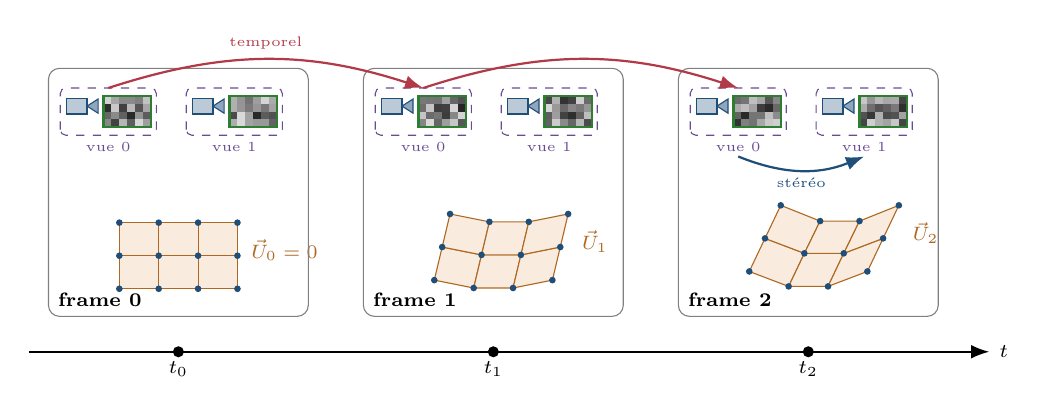
\begin{tikzpicture}
    \filldraw[fill=pyorange!15, draw=pyorange!80!black] (1.15,-0.75) -- (1.65,-0.75) -- (1.65,-0.33) -- (1.15,-0.33) -- cycle;
    \filldraw[fill=pyorange!15, draw=pyorange!80!black] (1.65,-0.75) -- (2.15,-0.75) -- (2.15,-0.33) -- (1.65,-0.33) -- cycle;
    \filldraw[fill=pyorange!15, draw=pyorange!80!black] (2.15,-0.75) -- (2.65,-0.75) -- (2.65,-0.33) -- (2.15,-0.33) -- cycle;
    \filldraw[fill=pyorange!15, draw=pyorange!80!black] (1.15,-0.33) -- (1.65,-0.33) -- (1.65,0.09) -- (1.15,0.09) -- cycle;
    \filldraw[fill=pyorange!15, draw=pyorange!80!black] (1.65,-0.33) -- (2.15,-0.33) -- (2.15,0.09) -- (1.65,0.09) -- cycle;
    \filldraw[fill=pyorange!15, draw=pyorange!80!black] (2.15,-0.33) -- (2.65,-0.33) -- (2.65,0.09) -- (2.15,0.09) -- cycle;
    \fill[pyblue] (1.15,-0.75) circle (1.2pt);
    \fill[pyblue] (1.65,-0.75) circle (1.2pt);
    \fill[pyblue] (2.15,-0.75) circle (1.2pt);
    \fill[pyblue] (2.65,-0.75) circle (1.2pt);
    \fill[pyblue] (1.15,-0.33) circle (1.2pt);
    \fill[pyblue] (1.65,-0.33) circle (1.2pt);
    \fill[pyblue] (2.15,-0.33) circle (1.2pt);
    \fill[pyblue] (2.65,-0.33) circle (1.2pt);
    \fill[pyblue] (1.15,0.09) circle (1.2pt);
    \fill[pyblue] (1.65,0.09) circle (1.2pt);
    \fill[pyblue] (2.15,0.09) circle (1.2pt);
    \fill[pyblue] (2.65,0.09) circle (1.2pt);
    \node[font=\scriptsize, text=pyorange!80!black, anchor=west] at (2.70,-0.26) {$\vec{U}_0 = 0$};
    \filldraw[fill=pyblue!30, draw=pyblue] (0.48,1.47) rectangle ++(0.26,0.2);
    \filldraw[fill=pyblue!50, draw=pyblue] (0.74,1.57) -- ++(0.14,0.09) -- ++(0,-0.18) -- cycle;
    \fill[black!47] (0.95,1.30) rectangle ++(0.1,0.1);
    \fill[black!60] (0.95,1.40) rectangle ++(0.1,0.1);
    \fill[black!82] (0.95,1.50) rectangle ++(0.1,0.1);
    \fill[black!18] (0.95,1.60) rectangle ++(0.1,0.1);
    \fill[black!74] (1.05,1.30) rectangle ++(0.1,0.1);
    \fill[black!46] (1.05,1.40) rectangle ++(0.1,0.1);
    \fill[black!21] (1.05,1.50) rectangle ++(0.1,0.1);
    \fill[black!35] (1.05,1.60) rectangle ++(0.1,0.1);
    \fill[black!29] (1.15,1.30) rectangle ++(0.1,0.1);
    \fill[black!62] (1.15,1.40) rectangle ++(0.1,0.1);
    \fill[black!75] (1.15,1.50) rectangle ++(0.1,0.1);
    \fill[black!46] (1.15,1.60) rectangle ++(0.1,0.1);
    \fill[black!63] (1.25,1.30) rectangle ++(0.1,0.1);
    \fill[black!84] (1.25,1.40) rectangle ++(0.1,0.1);
    \fill[black!28] (1.25,1.50) rectangle ++(0.1,0.1);
    \fill[black!46] (1.25,1.60) rectangle ++(0.1,0.1);
    \fill[black!16] (1.35,1.30) rectangle ++(0.1,0.1);
    \fill[black!42] (1.35,1.40) rectangle ++(0.1,0.1);
    \fill[black!67] (1.35,1.50) rectangle ++(0.1,0.1);
    \fill[black!50] (1.35,1.60) rectangle ++(0.1,0.1);
    \fill[black!38] (1.45,1.30) rectangle ++(0.1,0.1);
    \fill[black!64] (1.45,1.40) rectangle ++(0.1,0.1);
    \fill[black!35] (1.45,1.50) rectangle ++(0.1,0.1);
    \fill[black!24] (1.45,1.60) rectangle ++(0.1,0.1);
    \draw[pygreen, thick] (0.95,1.30) rectangle ++(0.6,0.4);
    \draw[pypurple, dashed, rounded corners=2pt] (0.40,1.20) rectangle (1.62,1.80);
    \coordinate (v00) at (1.01,1.80);
    \coordinate (b00) at (1.01,0.93);
    \node[font=\tiny, text=pypurple] at (1.01,1.05) {vue 0};
    \filldraw[fill=pyblue!30, draw=pyblue] (2.08,1.47) rectangle ++(0.26,0.2);
    \filldraw[fill=pyblue!50, draw=pyblue] (2.34,1.57) -- ++(0.14,0.09) -- ++(0,-0.18) -- cycle;
    \fill[black!32] (2.55,1.30) rectangle ++(0.1,0.1);
    \fill[black!71] (2.55,1.40) rectangle ++(0.1,0.1);
    \fill[black!31] (2.55,1.50) rectangle ++(0.1,0.1);
    \fill[black!31] (2.55,1.60) rectangle ++(0.1,0.1);
    \fill[black!15] (2.65,1.30) rectangle ++(0.1,0.1);
    \fill[black!15] (2.65,1.40) rectangle ++(0.1,0.1);
    \fill[black!41] (2.65,1.50) rectangle ++(0.1,0.1);
    \fill[black!42] (2.65,1.60) rectangle ++(0.1,0.1);
    \fill[black!36] (2.75,1.30) rectangle ++(0.1,0.1);
    \fill[black!36] (2.75,1.40) rectangle ++(0.1,0.1);
    \fill[black!52] (2.75,1.50) rectangle ++(0.1,0.1);
    \fill[black!55] (2.75,1.60) rectangle ++(0.1,0.1);
    \fill[black!40] (2.85,1.30) rectangle ++(0.1,0.1);
    \fill[black!84] (2.85,1.40) rectangle ++(0.1,0.1);
    \fill[black!41] (2.85,1.50) rectangle ++(0.1,0.1);
    \fill[black!38] (2.85,1.60) rectangle ++(0.1,0.1);
    \fill[black!40] (2.95,1.30) rectangle ++(0.1,0.1);
    \fill[black!64] (2.95,1.40) rectangle ++(0.1,0.1);
    \fill[black!53] (2.95,1.50) rectangle ++(0.1,0.1);
    \fill[black!17] (2.95,1.60) rectangle ++(0.1,0.1);
    \fill[black!61] (3.05,1.30) rectangle ++(0.1,0.1);
    \fill[black!68] (3.05,1.40) rectangle ++(0.1,0.1);
    \fill[black!36] (3.05,1.50) rectangle ++(0.1,0.1);
    \fill[black!33] (3.05,1.60) rectangle ++(0.1,0.1);
    \draw[pygreen, thick] (2.55,1.30) rectangle ++(0.6,0.4);
    \draw[pypurple, dashed, rounded corners=2pt] (2.00,1.20) rectangle (3.22,1.80);
    \coordinate (v01) at (2.61,1.80);
    \coordinate (b01) at (2.61,0.93);
    \node[font=\tiny, text=pypurple] at (2.61,1.05) {vue 1};
    \draw[gray, rounded corners] (0.25,-1.1) rectangle (3.55,2.05);
    \node[font=\scriptsize\bfseries, anchor=south west] at (0.25,-1.1) {frame 0};
    \fill (1.90,-1.55) circle (2pt) node[below, font=\scriptsize] {$t_0$};
    \filldraw[fill=pyorange!15, draw=pyorange!80!black] (5.15,-0.64) -- (5.65,-0.74) -- (5.75,-0.32) -- (5.25,-0.22) -- cycle;
    \filldraw[fill=pyorange!15, draw=pyorange!80!black] (5.65,-0.74) -- (6.15,-0.74) -- (6.25,-0.32) -- (5.75,-0.32) -- cycle;
    \filldraw[fill=pyorange!15, draw=pyorange!80!black] (6.15,-0.74) -- (6.65,-0.64) -- (6.75,-0.22) -- (6.25,-0.32) -- cycle;
    \filldraw[fill=pyorange!15, draw=pyorange!80!black] (5.25,-0.22) -- (5.75,-0.32) -- (5.85,0.10) -- (5.35,0.20) -- cycle;
    \filldraw[fill=pyorange!15, draw=pyorange!80!black] (5.75,-0.32) -- (6.25,-0.32) -- (6.35,0.10) -- (5.85,0.10) -- cycle;
    \filldraw[fill=pyorange!15, draw=pyorange!80!black] (6.25,-0.32) -- (6.75,-0.22) -- (6.85,0.20) -- (6.35,0.10) -- cycle;
    \fill[pyblue] (5.15,-0.64) circle (1.2pt);
    \fill[pyblue] (5.65,-0.74) circle (1.2pt);
    \fill[pyblue] (6.15,-0.74) circle (1.2pt);
    \fill[pyblue] (6.65,-0.64) circle (1.2pt);
    \fill[pyblue] (5.25,-0.22) circle (1.2pt);
    \fill[pyblue] (5.75,-0.32) circle (1.2pt);
    \fill[pyblue] (6.25,-0.32) circle (1.2pt);
    \fill[pyblue] (6.75,-0.22) circle (1.2pt);
    \fill[pyblue] (5.35,0.20) circle (1.2pt);
    \fill[pyblue] (5.85,0.10) circle (1.2pt);
    \fill[pyblue] (6.35,0.10) circle (1.2pt);
    \fill[pyblue] (6.85,0.20) circle (1.2pt);
    \node[font=\scriptsize, text=pyorange!80!black, anchor=west] at (6.90,-0.15) {$\vec{U}_1$};
    \filldraw[fill=pyblue!30, draw=pyblue] (4.48,1.47) rectangle ++(0.26,0.2);
    \filldraw[fill=pyblue!50, draw=pyblue] (4.74,1.57) -- ++(0.14,0.09) -- ++(0,-0.18) -- cycle;
    \fill[black!48] (4.95,1.30) rectangle ++(0.1,0.1);
    \fill[black!23] (4.95,1.40) rectangle ++(0.1,0.1);
    \fill[black!57] (4.95,1.50) rectangle ++(0.1,0.1);
    \fill[black!53] (4.95,1.60) rectangle ++(0.1,0.1);
    \fill[black!15] (5.05,1.30) rectangle ++(0.1,0.1);
    \fill[black!58] (5.05,1.40) rectangle ++(0.1,0.1);
    \fill[black!23] (5.05,1.50) rectangle ++(0.1,0.1);
    \fill[black!54] (5.05,1.60) rectangle ++(0.1,0.1);
    \fill[black!60] (5.15,1.30) rectangle ++(0.1,0.1);
    \fill[black!54] (5.15,1.40) rectangle ++(0.1,0.1);
    \fill[black!76] (5.15,1.50) rectangle ++(0.1,0.1);
    \fill[black!55] (5.15,1.60) rectangle ++(0.1,0.1);
    \fill[black!38] (5.25,1.30) rectangle ++(0.1,0.1);
    \fill[black!76] (5.25,1.40) rectangle ++(0.1,0.1);
    \fill[black!75] (5.25,1.50) rectangle ++(0.1,0.1);
    \fill[black!37] (5.25,1.60) rectangle ++(0.1,0.1);
    \fill[black!22] (5.35,1.30) rectangle ++(0.1,0.1);
    \fill[black!47] (5.35,1.40) rectangle ++(0.1,0.1);
    \fill[black!17] (5.35,1.50) rectangle ++(0.1,0.1);
    \fill[black!60] (5.35,1.60) rectangle ++(0.1,0.1);
    \fill[black!66] (5.45,1.30) rectangle ++(0.1,0.1);
    \fill[black!17] (5.45,1.40) rectangle ++(0.1,0.1);
    \fill[black!85] (5.45,1.50) rectangle ++(0.1,0.1);
    \fill[black!68] (5.45,1.60) rectangle ++(0.1,0.1);
    \draw[pygreen, thick] (4.95,1.30) rectangle ++(0.6,0.4);
    \draw[pypurple, dashed, rounded corners=2pt] (4.40,1.20) rectangle (5.62,1.80);
    \coordinate (v10) at (5.01,1.80);
    \coordinate (b10) at (5.01,0.93);
    \node[font=\tiny, text=pypurple] at (5.01,1.05) {vue 0};
    \filldraw[fill=pyblue!30, draw=pyblue] (6.08,1.47) rectangle ++(0.26,0.2);
    \filldraw[fill=pyblue!50, draw=pyblue] (6.34,1.57) -- ++(0.14,0.09) -- ++(0,-0.18) -- cycle;
    \fill[black!61] (6.55,1.30) rectangle ++(0.1,0.1);
    \fill[black!63] (6.55,1.40) rectangle ++(0.1,0.1);
    \fill[black!16] (6.55,1.50) rectangle ++(0.1,0.1);
    \fill[black!72] (6.55,1.60) rectangle ++(0.1,0.1);
    \fill[black!20] (6.65,1.30) rectangle ++(0.1,0.1);
    \fill[black!38] (6.65,1.40) rectangle ++(0.1,0.1);
    \fill[black!40] (6.65,1.50) rectangle ++(0.1,0.1);
    \fill[black!30] (6.65,1.60) rectangle ++(0.1,0.1);
    \fill[black!46] (6.75,1.30) rectangle ++(0.1,0.1);
    \fill[black!74] (6.75,1.40) rectangle ++(0.1,0.1);
    \fill[black!59] (6.75,1.50) rectangle ++(0.1,0.1);
    \fill[black!80] (6.75,1.60) rectangle ++(0.1,0.1);
    \fill[black!60] (6.85,1.30) rectangle ++(0.1,0.1);
    \fill[black!82] (6.85,1.40) rectangle ++(0.1,0.1);
    \fill[black!47] (6.85,1.50) rectangle ++(0.1,0.1);
    \fill[black!74] (6.85,1.60) rectangle ++(0.1,0.1);
    \fill[black!28] (6.95,1.30) rectangle ++(0.1,0.1);
    \fill[black!62] (6.95,1.40) rectangle ++(0.1,0.1);
    \fill[black!52] (6.95,1.50) rectangle ++(0.1,0.1);
    \fill[black!19] (6.95,1.60) rectangle ++(0.1,0.1);
    \fill[black!70] (7.05,1.30) rectangle ++(0.1,0.1);
    \fill[black!26] (7.05,1.40) rectangle ++(0.1,0.1);
    \fill[black!41] (7.05,1.50) rectangle ++(0.1,0.1);
    \fill[black!58] (7.05,1.60) rectangle ++(0.1,0.1);
    \draw[pygreen, thick] (6.55,1.30) rectangle ++(0.6,0.4);
    \draw[pypurple, dashed, rounded corners=2pt] (6.00,1.20) rectangle (7.22,1.80);
    \coordinate (v11) at (6.61,1.80);
    \coordinate (b11) at (6.61,0.93);
    \node[font=\tiny, text=pypurple] at (6.61,1.05) {vue 1};
    \draw[gray, rounded corners] (4.25,-1.1) rectangle (7.55,2.05);
    \node[font=\scriptsize\bfseries, anchor=south west] at (4.25,-1.1) {frame 1};
    \fill (5.90,-1.55) circle (2pt) node[below, font=\scriptsize] {$t_1$};
    \filldraw[fill=pyorange!15, draw=pyorange!80!black] (9.15,-0.53) -- (9.65,-0.72) -- (9.85,-0.30) -- (9.35,-0.11) -- cycle;
    \filldraw[fill=pyorange!15, draw=pyorange!80!black] (9.65,-0.72) -- (10.15,-0.72) -- (10.35,-0.30) -- (9.85,-0.30) -- cycle;
    \filldraw[fill=pyorange!15, draw=pyorange!80!black] (10.15,-0.72) -- (10.65,-0.53) -- (10.85,-0.11) -- (10.35,-0.30) -- cycle;
    \filldraw[fill=pyorange!15, draw=pyorange!80!black] (9.35,-0.11) -- (9.85,-0.30) -- (10.05,0.11) -- (9.55,0.31) -- cycle;
    \filldraw[fill=pyorange!15, draw=pyorange!80!black] (9.85,-0.30) -- (10.35,-0.30) -- (10.55,0.11) -- (10.05,0.11) -- cycle;
    \filldraw[fill=pyorange!15, draw=pyorange!80!black] (10.35,-0.30) -- (10.85,-0.11) -- (11.05,0.31) -- (10.55,0.11) -- cycle;
    \fill[pyblue] (9.15,-0.53) circle (1.2pt);
    \fill[pyblue] (9.65,-0.72) circle (1.2pt);
    \fill[pyblue] (10.15,-0.72) circle (1.2pt);
    \fill[pyblue] (10.65,-0.53) circle (1.2pt);
    \fill[pyblue] (9.35,-0.11) circle (1.2pt);
    \fill[pyblue] (9.85,-0.30) circle (1.2pt);
    \fill[pyblue] (10.35,-0.30) circle (1.2pt);
    \fill[pyblue] (10.85,-0.11) circle (1.2pt);
    \fill[pyblue] (9.55,0.31) circle (1.2pt);
    \fill[pyblue] (10.05,0.11) circle (1.2pt);
    \fill[pyblue] (10.55,0.11) circle (1.2pt);
    \fill[pyblue] (11.05,0.31) circle (1.2pt);
    \node[font=\scriptsize, text=pyorange!80!black, anchor=west] at (11.10,-0.04) {$\vec{U}_2$};
    \filldraw[fill=pyblue!30, draw=pyblue] (8.48,1.47) rectangle ++(0.26,0.2);
    \filldraw[fill=pyblue!50, draw=pyblue] (8.74,1.57) -- ++(0.14,0.09) -- ++(0,-0.18) -- cycle;
    \fill[black!80] (8.95,1.30) rectangle ++(0.1,0.1);
    \fill[black!61] (8.95,1.40) rectangle ++(0.1,0.1);
    \fill[black!33] (8.95,1.50) rectangle ++(0.1,0.1);
    \fill[black!58] (8.95,1.60) rectangle ++(0.1,0.1);
    \fill[black!50] (9.05,1.30) rectangle ++(0.1,0.1);
    \fill[black!84] (9.05,1.40) rectangle ++(0.1,0.1);
    \fill[black!26] (9.05,1.50) rectangle ++(0.1,0.1);
    \fill[black!54] (9.05,1.60) rectangle ++(0.1,0.1);
    \fill[black!55] (9.15,1.30) rectangle ++(0.1,0.1);
    \fill[black!54] (9.15,1.40) rectangle ++(0.1,0.1);
    \fill[black!37] (9.15,1.50) rectangle ++(0.1,0.1);
    \fill[black!25] (9.15,1.60) rectangle ++(0.1,0.1);
    \fill[black!34] (9.25,1.30) rectangle ++(0.1,0.1);
    \fill[black!54] (9.25,1.40) rectangle ++(0.1,0.1);
    \fill[black!76] (9.25,1.50) rectangle ++(0.1,0.1);
    \fill[black!35] (9.25,1.60) rectangle ++(0.1,0.1);
    \fill[black!21] (9.35,1.30) rectangle ++(0.1,0.1);
    \fill[black!25] (9.35,1.40) rectangle ++(0.1,0.1);
    \fill[black!83] (9.35,1.50) rectangle ++(0.1,0.1);
    \fill[black!66] (9.35,1.60) rectangle ++(0.1,0.1);
    \fill[black!19] (9.45,1.30) rectangle ++(0.1,0.1);
    \fill[black!45] (9.45,1.40) rectangle ++(0.1,0.1);
    \fill[black!59] (9.45,1.50) rectangle ++(0.1,0.1);
    \fill[black!47] (9.45,1.60) rectangle ++(0.1,0.1);
    \draw[pygreen, thick] (8.95,1.30) rectangle ++(0.6,0.4);
    \draw[pypurple, dashed, rounded corners=2pt] (8.40,1.20) rectangle (9.62,1.80);
    \coordinate (v20) at (9.01,1.80);
    \coordinate (b20) at (9.01,0.93);
    \node[font=\tiny, text=pypurple] at (9.01,1.05) {vue 0};
    \filldraw[fill=pyblue!30, draw=pyblue] (10.08,1.47) rectangle ++(0.26,0.2);
    \filldraw[fill=pyblue!50, draw=pyblue] (10.34,1.57) -- ++(0.14,0.09) -- ++(0,-0.18) -- cycle;
    \fill[black!73] (10.55,1.30) rectangle ++(0.1,0.1);
    \fill[black!68] (10.55,1.40) rectangle ++(0.1,0.1);
    \fill[black!33] (10.55,1.50) rectangle ++(0.1,0.1);
    \fill[black!22] (10.55,1.60) rectangle ++(0.1,0.1);
    \fill[black!19] (10.65,1.30) rectangle ++(0.1,0.1);
    \fill[black!78] (10.65,1.40) rectangle ++(0.1,0.1);
    \fill[black!57] (10.65,1.50) rectangle ++(0.1,0.1);
    \fill[black!41] (10.65,1.60) rectangle ++(0.1,0.1);
    \fill[black!31] (10.75,1.30) rectangle ++(0.1,0.1);
    \fill[black!31] (10.75,1.40) rectangle ++(0.1,0.1);
    \fill[black!67] (10.75,1.50) rectangle ++(0.1,0.1);
    \fill[black!28] (10.75,1.60) rectangle ++(0.1,0.1);
    \fill[black!36] (10.85,1.30) rectangle ++(0.1,0.1);
    \fill[black!70] (10.85,1.40) rectangle ++(0.1,0.1);
    \fill[black!62] (10.85,1.50) rectangle ++(0.1,0.1);
    \fill[black!34] (10.85,1.60) rectangle ++(0.1,0.1);
    \fill[black!22] (10.95,1.30) rectangle ++(0.1,0.1);
    \fill[black!68] (10.95,1.40) rectangle ++(0.1,0.1);
    \fill[black!52] (10.95,1.50) rectangle ++(0.1,0.1);
    \fill[black!33] (10.95,1.60) rectangle ++(0.1,0.1);
    \fill[black!73] (11.05,1.30) rectangle ++(0.1,0.1);
    \fill[black!36] (11.05,1.40) rectangle ++(0.1,0.1);
    \fill[black!81] (11.05,1.50) rectangle ++(0.1,0.1);
    \fill[black!73] (11.05,1.60) rectangle ++(0.1,0.1);
    \draw[pygreen, thick] (10.55,1.30) rectangle ++(0.6,0.4);
    \draw[pypurple, dashed, rounded corners=2pt] (10.00,1.20) rectangle (11.22,1.80);
    \coordinate (v21) at (10.61,1.80);
    \coordinate (b21) at (10.61,0.93);
    \node[font=\tiny, text=pypurple] at (10.61,1.05) {vue 1};
    \draw[gray, rounded corners] (8.25,-1.1) rectangle (11.55,2.05);
    \node[font=\scriptsize\bfseries, anchor=south west] at (8.25,-1.1) {frame 2};
    \fill (9.90,-1.55) circle (2pt) node[below, font=\scriptsize] {$t_2$};
    \draw[->, thick] (0,-1.55) -- (12.2,-1.55) node[right, font=\scriptsize]{$t$};
    % Exemples d'appariements
    \draw[->, thick, pyred] (v00) to[bend left=18] node[above, font=\tiny]{temporel} (v10);
    \draw[->, thick, pyred] (v10) to[bend left=18] (v20);
    \draw[->, thick, pyblue] (b20) to[bend right=22] node[below=-1pt, font=\tiny]{stéréo} (b21);
  \end{tikzpicture}}
 
  \smallskip
  \scriptsize
  \begin{tabular}{@{}r@{\quad}l@{}}
    \textbf{Maillage} & \textcolor{pyorange}{$\blacksquare$} un seul maillage de référence, déformé
      par un déplacement $\vec{U}_f$ par frame \\
    \textbf{Vues} & \textcolor{pypurple}{$\square$} par frame, des vues :
      \textcolor{pyblue}{caméra} + \textcolor{pygreen}{image} \\
    \textbf{Appariements} & \textcolor{pyred}{$\rightarrow$} temporel,
      \textcolor{pyblue}{$\rightarrow$} stéréo : les vues comparées \\
  \end{tabular}
 
  \smallskip
  \small On cherche les $\vec{U}_f$ (et des paramètres de caméras) qui rendent les vues
  \alert{cohérentes}.
\end{frame}

% ---------------------------------------------------------------------
\begin{frame}{\texttt{SDICAnalysis} : comment les données s'emboîtent}
  \centering
  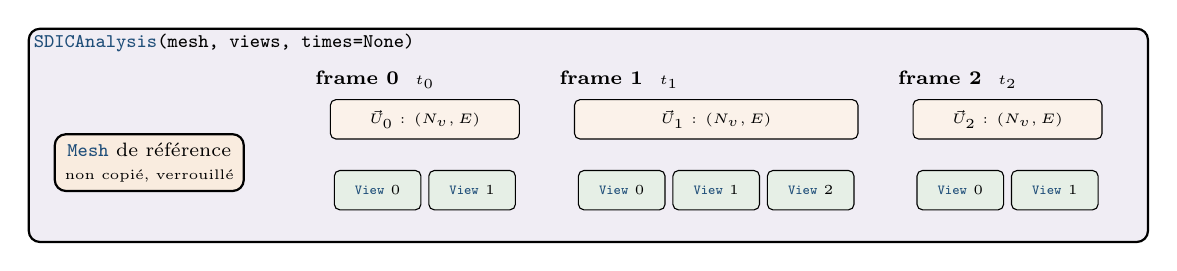
\begin{tikzpicture}
    \node[box, fill=pyorange!15, minimum width=2.4cm] (mesh) at (-0.9,0) {\cls{Mesh} de référence\\\tiny non copié, verrouillé};
    % frame 0 : 2 vues
    \node[attr, fill=pyorange!10, minimum width=2.4cm] (U0) at (2.6,0.55) {$\vec{U}_0$ : $(N_v, E)$};
    \node[attr, fill=pygreen!12, minimum width=1.1cm] (V00) at (2.0,-0.35) {\cls{View} 0};
    \node[attr, fill=pygreen!12, minimum width=1.1cm] (V01) at (3.2,-0.35) {\cls{View} 1};
    % frame 1 : 3 vues
    \node[attr, fill=pyorange!10, minimum width=3.6cm] (U1) at (6.3,0.55) {$\vec{U}_1$ : $(N_v, E)$};
    \node[attr, fill=pygreen!12, minimum width=1.1cm] (V10) at (5.1,-0.35) {\cls{View} 0};
    \node[attr, fill=pygreen!12, minimum width=1.1cm] (V11) at (6.3,-0.35) {\cls{View} 1};
    \node[attr, fill=pygreen!12, minimum width=1.1cm] (V12) at (7.5,-0.35) {\cls{View} 2};
    % frame 2 : 2 vues
    \node[attr, fill=pyorange!10, minimum width=2.4cm] (U2) at (10.0,0.55) {$\vec{U}_2$ : $(N_v, E)$};
    \node[attr, fill=pygreen!12, minimum width=1.1cm] (V20) at (9.4,-0.35) {\cls{View} 0};
    \node[attr, fill=pygreen!12, minimum width=1.1cm] (V21) at (10.6,-0.35) {\cls{View} 1};
    \begin{scope}[on background layer]
      \node[container, fill=white, fit=(U0)(V00)(V01), inner ysep=9pt, yshift=3pt] (F0) {};
      \node[container, fill=white, fit=(U1)(V10)(V12), inner ysep=9pt, yshift=3pt] (F1) {};
      \node[container, fill=white, fit=(U2)(V20)(V21), inner ysep=9pt, yshift=3pt] (F2) {};
    \end{scope}
    \node[ctitle] at (F0.north west) {frame 0 \ \tiny $t_0$};
    \node[ctitle] at (F1.north west) {frame 1 \ \tiny $t_1$};
    \node[ctitle] at (F2.north west) {frame 2 \ \tiny $t_2$};
    \begin{scope}[on background layer]
      \node[container, fill=pypurple!10, fit=(mesh)(F0)(F2), inner sep=9pt, yshift=4pt] (analysis) {};
    \end{scope}
    \node[ctitle] at (analysis.north west) {\cls{SDICAnalysis}\code{(mesh, views, times=None)}};
  \end{tikzpicture}
 
  \medskip
  \footnotesize
  \begin{itemize}\setlength{\itemsep}{1pt}
    \item les déplacements sont stockés \alert{hors du maillage}, un tableau par frame
          (lecture seule, jamais remis à \code{None}) ;
    \item instants d'acquisition \code{times} optionnels, strictement croissants ;
    \item le \alert{nombre de vues} peut changer d'une frame à l'autre (même zéro) ;
    \item des vues peuvent partager, ou non, la même \cls{Camera}, la même \cls{Image},
          ou seulement une \alert{transformation} (extrinsèque, distorsion, intrinsèque) ;
    \item chaque transformation distincte est repérée par \code{(kind, index)} :
          \code{analysis.display\_structure("distortion")},
          \code{analysis.get\_transformation("distortion", 1)}.
  \end{itemize}
\end{frame}

% ---------------------------------------------------------------------
\begin{frame}[fragile]{\texttt{SDICAnalysis} dans le code}
  \begin{columns}[T]
    \begin{column}{0.52\textwidth}
\begin{lstlisting}[basicstyle=\ttfamily\tiny]
from pysdic import SDICAnalysis, View
 
# views[f] : les vues de la frame f
views = [[View(left, images[f, 0]), View(right, images[f, 1])]
         for f in range(2)]
analysis = SDICAnalysis(mesh, views, times=[0.0, 0.1])
analysis.set_zero_displacement(0)
analysis.set_displacement(1, first_guess)
 
analysis.get_view(1, 0)        # frame 1, vue 0
analysis.get_displacement(1)   # (N_v, 3), lecture seule
analysis.get_deformed_mesh(1)  # Mesh déformé
 
analysis.display_structure("extrinsic")
#   Frame 0  : [0, 1]
#   Frame 1  : [0, 1]
p = analysis.get_transformation_parameters("extrinsic", 1)
analysis.set_transformation_parameters("extrinsic", 1, p)
 
# Une autre structure = une nouvelle analyse
other = analysis.with_frame_views(1, [View(left, image)])
other = analysis.with_mesh(finer_mesh, keep_displacements=False)
\end{lstlisting}
    \end{column}
    \begin{column}{0.46\textwidth}\scriptsize
      \begin{itemize}\setlength{\itemsep}{1pt}
        \item vues données \alert{à la construction} : la structure est figée,
              calculée une fois ;
        \item \texttt{with\_mesh}, \texttt{with\_views}, \texttt{with\_frame\_views},
              \texttt{with\_times} : nouvelle \cls{SDICAnalysis} qui \alert{partage} le reste
              (images, caméras, déplacements) ;
        \item \texttt{compute\_structure(kind)}, par \alert{identité} :
              vue, image, caméra, extrinsèque, distorsion, intrinsèque ;
        \item \texttt{get/set\_transformation\_parameters} : les paramètres restent
              modifiables, verrous respectés ;
        \item \texttt{check\_consistency} (à la construction) : extrinsèques,
              distorsions et intrinsèques \alert{disjoints}, et chaque
              transformation unitaire présente \alert{une seule fois} (même dans
              une composition ou une reparamétrisation).
      \end{itemize}
    \end{column}
  \end{columns}
\end{frame}

% ---------------------------------------------------------------------
\begin{frame}[fragile]{Montages types}
  \begin{columns}[T]
    \begin{column}{0.53\textwidth}
\begin{lstlisting}[basicstyle=\ttfamily\tiny]
from pysdic import (create_multicamera_analysis, create_bicamera_analysis,
                    create_splitscreen_analysis, create_cordin_analysis)
 
# images[i][f] : caméra i, frame f
analysis = create_multicamera_analysis(mesh, cameras, images,
                                       times=times)  # optionnel
analysis = create_bicamera_analysis(mesh, left, right, imgs_g, imgs_d)
 
# Une image par frame, partagée par les vues
analysis = create_splitscreen_analysis(mesh, [left, right], images)
 
# Une distorsion par frame (miroir tournant)
analysis = create_cordin_analysis(mesh,
    extrinsics=[ext_g, ext_d],
    intrinsic=PinholeIntrinsic.from_matrix(K),
    distortions=[BrownDistortion(d) for d in ds],
    images=images)
\end{lstlisting}
    \end{column}
    \begin{column}{0.45\textwidth}\footnotesize
      \textbf{Cordin} :
      \[
        \text{Cam.}[i][f] = \text{Intr.} \circ \text{Dist.}[f] \circ \text{Extr.}[i]
      \]
      \begin{itemize}
        \item transformations \alert{non copiées} : modifier une distorsion
              modifie toutes les caméras de sa frame ;
        \item déplacements non définis à la création.
      \end{itemize}
    \end{column}
  \end{columns}
\end{frame}

% ---------------------------------------------------------------------
\begin{frame}[fragile]{Sauvegarder une analyse}
  \begin{columns}[T]
    \begin{column}{0.44\textwidth}
\begin{lstlisting}[language={},basicstyle=\ttfamily\tiny]
essai/
  metadata.json   # format, version, date, titre
  README.txt
  manifest.json   # SHA-256 de chaque fichier
  structure.json  # caméras, vues, frames
  mesh/mesh.npz   # (+ mesh.vtk, export)
  images/image_00.npz ...
  extrinsics/extrinsic_0.json ...
  distortions/distortion_0.json ...
  intrinsics/intrinsic_0.json ...
  displacements.npz   # frame_00, ...
  times.npz
\end{lstlisting}
\begin{lstlisting}[basicstyle=\ttfamily\tiny]
analysis.to_folder("essai", title="Essai 3",
                   export_vtk=True)
analysis = SDICAnalysis.from_folder("essai")
 
analysis.to_archive("essai.zip", overwrite=True)
analysis = SDICAnalysis.from_archive("essai.zip")
\end{lstlisting}
    \end{column}
    \begin{column}{0.54\textwidth}\scriptsize
      \begin{itemize}\setlength{\itemsep}{1pt}
        \item chaque \alert{atome} (image, transformation) écrit \alert{une seule fois},
              même partagé ; \texttt{structure.json} relie caméras, vues et frames ;
        \item numéros sur autant de chiffres que le plus grand indice :
              1543 images $\to$ \texttt{image\_0000.npz} ;
        \item \alert{aucun pickle} : JSON et tableaux numériques
              (\texttt{allow\_pickle=False}) ;
        \item écriture \alert{atomique} : dossier temporaire horodaté, puis renommé ;
              \texttt{overwrite=True} ne remplace qu'une sauvegarde \cls{SDICAnalysis} ;
        \item lecture : format, version, SHA-256 (\texttt{check\_integrity}), puis
              structures comparées $\to$ erreur \alert{« Inconsistent loading »} ;
        \item archive : les mêmes fichiers dans un zip (\texttt{compress=False} par
              défaut) ; chemins dangereux refusés.
      \end{itemize}
      \scriptsize Non sauvegardés : points d'intégration et appariements.
    \end{column}
  \end{columns}
\end{frame}

% ---------------------------------------------------------------------
\begin{frame}[fragile]{\texttt{SDICUnknowns} : les inconnues $[\vec{p}_U,\ \vec{p}_T]$}
  \begin{columns}[T]
    \begin{column}{0.49\textwidth}\footnotesize
      \begin{center}
      \scriptsize
      \begin{tabular}{lll}
        \toprule
        problème & frames & transformations \\
        \midrule
        mesure     & \code{[1]} & \code{[]} \\
        étalonnage & \code{[]}  & \code{[("extrinsic", 1)]} \\
        conjoint   & \code{[1]} & \code{[("distortion", 1)]} \\
        \bottomrule
      \end{tabular}
      \end{center}
      \scriptsize
      \begin{itemize}\setlength{\itemsep}{1pt}
        \item $\vec{p}_U$ : déplacements des frames optimisées, en \alert{ordre
              Fortran} ($[U^x_{1..N_v}, U^y_{1..N_v}, U^z_{1..N_v}]$) ;
        \item $\vec{p}_T$ : paramètres des transformations optimisées ;
        \item \alert{simple description} (comme \cls{Pairing}) : ne connaît
              \alert{pas} l'analyse, validée par \texttt{analysis.validate\_unknowns} ;
        \item le vecteur est construit par l'analyse :
              \texttt{analysis.pack/unpack/apply\_unknowns(unknowns, ...)} ;
        \item avec paramétrisation : \textcolor{pyred}{\textbf{il FAUT}
              \texttt{param.reparametrized\_pack/unpack/apply}}.
      \end{itemize}
    \end{column}
    \begin{column}{0.49\textwidth}
\begin{lstlisting}[basicstyle=\ttfamily\tiny]
from pysdic import SDICUnknowns
 
unknowns = SDICUnknowns([1], [("distortion", 1)])
analysis.validate_unknowns(unknowns)
analysis.n_unknowns(unknowns)
p0 = analysis.pack_unknowns(unknowns)        # état -> p
U, T = analysis.unpack_unknowns(unknowns, p) # p -> copies
U[1]                                         # (N_v, E)
T[("distortion", 1)]                         # (n_p,)
analysis.apply_unknowns(unknowns, p)         # p -> analyse
 
analysis.get_unknowns_frame_slice(unknowns, 1)
analysis.get_unknowns_transformation_slice(
    unknowns, "distortion", 1)
analysis.compute_unknowns_indices(
    unknowns, vertices=v, components=[0, 1])
\end{lstlisting}
      \scriptsize \textcolor{pyred}{Attention :} déplacements et transformations ne
      sont pas toujours séparables (un mouvement rigide de la surface équivaut à un
      mouvement rigide de toutes les caméras). N'optimiser que ce que les
      appariements déterminent.
    \end{column}
  \end{columns}
\end{frame}

% ---------------------------------------------------------------------
\begin{frame}{Le problème : comparer des vues par paires}
  \small
  Un \alert{appariement} relie la vue $(f_1, v_1)$ à la vue $(f_2, v_2)$. Pour un point
  matériel $\vec{X}_p$ de poids $w_p$ :
  \[
    r_p = \sqrt{w_p}\,\Bigl( [I_2 \circ P_2^{\vec{p}_T}]\bigl(\vec{X}_p + \vec{u}_{f_2}(\vec{X}_p)\bigr)
          - [I_1 \circ P_1^{\vec{p}_T}]\bigl(\vec{X}_p + \vec{u}_{f_1}(\vec{X}_p)\bigr) \Bigr),
    \qquad
    \vec{u}_f(\vec{X}_p) = \sum_k N_k(\Xi_p)\,\vec{U}_{f,k}
  \]
  \[
    \Phi(\vec{p}_U, \vec{p}_T) = \sum_{\text{appariements}} \sum_p r_p^2,
    \qquad
    \vec{p}_U : \text{déplacements des sommets},\quad
    \vec{p}_T : \text{paramètres de caméras}
  \]
 
  \centering
  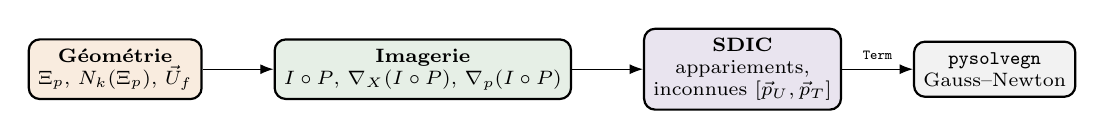
\begin{tikzpicture}
    \node[box, fill=pyorange!15] (g) {\textbf{Géométrie}\\$\Xi_p$, $N_k(\Xi_p)$, $\vec{U}_f$};
    \node[box, fill=pygreen!12, right=0.9cm of g] (i) {\textbf{Imagerie}\\$I \circ P$, $\nabla_X(I \circ P)$, $\nabla_p(I \circ P)$};
    \node[box, fill=pypurple!15, right=0.9cm of i] (s) {\textbf{SDIC}\\appariements,\\inconnues $[\vec{p}_U, \vec{p}_T]$};
    \node[box, fill=gray!10, right=0.9cm of s] (j) {\texttt{pysolvegn}\\Gauss--Newton};
    \draw[->] (g) -- (i); \draw[->] (i) -- (s); \draw[->] (s) -- node[above,font=\tiny]{\code{Term}} (j);
  \end{tikzpicture}
 
  \medskip
  \small Un seul terme, \cls{SDICCorrelationTerm}, optimise les déplacements, les
  paramètres des caméras, ou les deux à la fois.
\end{frame}

% ---------------------------------------------------------------------
\begin{frame}[fragile]{\texttt{Pairing} : quoi comparer}
  \begin{columns}[c]
    \begin{column}{0.52\textwidth}
      \centering
      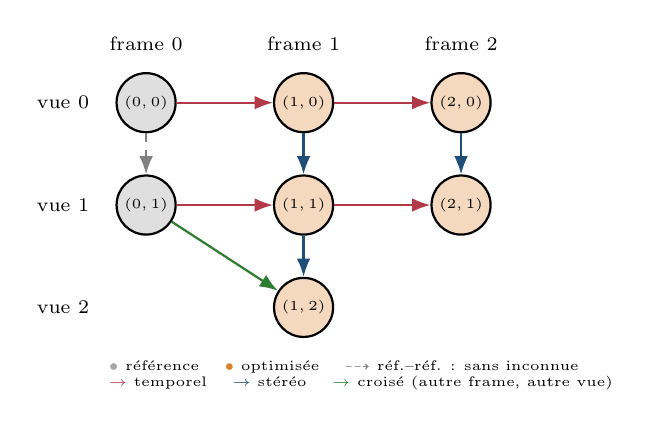
\begin{tikzpicture}[v/.style={circle, draw, thick, minimum size=0.75cm, font=\tiny, inner sep=0pt}]
        \foreach \f/\c in {0/gray!25, 1/pyorange!30, 2/pyorange!30}{
          \foreach \v in {0,1}{
            \node[v, fill=\c] (n\f\v) at (2.0*\f, -1.3*\v) {$(\f,\v)$};
          }
          \node[font=\scriptsize] at (2.0*\f, 0.75) {frame \f};
        }
        \node[v, fill=pyorange!30] (n12) at (2.0, -2.6) {$(1,2)$};
        \node[font=\scriptsize, anchor=east] at (-0.6,0) {vue 0};
        \node[font=\scriptsize, anchor=east] at (-0.6,-1.3) {vue 1};
        \node[font=\scriptsize, anchor=east] at (-0.6,-2.6) {vue 2};
        \draw[->,thick,pyred] (n00) -- (n10); \draw[->,thick,pyred] (n10) -- (n20);
        \draw[->,thick,pyred] (n01) -- (n11); \draw[->,thick,pyred] (n11) -- (n21);
        \draw[->,thick,pyblue] (n10) -- (n11); \draw[->,thick,pyblue] (n20) -- (n21);
        \draw[->,thick,pyblue] (n11) -- (n12);
        \draw[->,thick,pygreen] (n01) -- (n12);
        \draw[->,thick,gray,dashed] (n00) -- (n01);
        \node[font=\tiny, align=left, anchor=north west] at (-0.6,-3.15)
          {\textcolor{gray!70}{$\bullet$} référence \quad \textcolor{pyorange}{$\bullet$} optimisée
           \quad \textcolor{gray}{$\dashrightarrow$} réf.--réf. : sans inconnue\\
           \textcolor{pyred}{$\rightarrow$} temporel \quad \textcolor{pyblue}{$\rightarrow$} stéréo
           \quad \textcolor{pygreen}{$\rightarrow$} croisé (autre frame, autre vue)};
      \end{tikzpicture}
    \end{column}
    \begin{column}{0.46\textwidth}
\begin{lstlisting}[basicstyle=\ttfamily\tiny]
from pysdic import Pairing
 
Pairing(0, 0, 1, 0)   # f1, v1, f2, v2
Pairing.temporal(0, 0, 1)  # v0: f0->f1
Pairing.stereo(1, 0, 1)    # f1: v0->v1
Pairing(0, 1, 1, 2)        # croisé : accepté
pairing.is_stereo, pairing.reversed()
analysis.validate_pairing(pairing)  # vues, canaux
\end{lstlisting}
      \scriptsize Règles du terme de corrélation :
      \begin{itemize}
        \item frame non optimisée = \alert{référence} (déplacement fixé, défini) ;
        \item appariement \alert{sans inconnue} ignoré ; réf.--réf. utile en
              étalonnage (transformation optimisée) ;
        \item frame ou transformation optimisée sans appariement $\to$ erreur.
      \end{itemize}
    \end{column}
  \end{columns}
\end{frame}

% ---------------------------------------------------------------------
\begin{frame}[fragile]{\texttt{SDICCorrelationTerm} : un terme, trois problèmes}
  \begin{columns}[T]
    \begin{column}{0.53\textwidth}
\begin{lstlisting}[basicstyle=\ttfamily\tiny]
from pysdic import SDICCorrelationTerm, SDICUnknowns
 
unknowns = SDICUnknowns([1], [("distortion", 1)])
correlation = SDICCorrelationTerm(
    analysis, unknowns, ip, pairings,
    mode="rJ",                  # ou "gH"
    gl_correction={"mode": "ZNSSD"},
    use_cache=True)
 
result = pysolvegn.solve(terms=[correlation.term],
                         p0=correlation.pack())
correlation.apply(result.parameters)
 
# Frame suivante : nouvelles inconnues -> nouveau terme
unknowns_2 = SDICUnknowns([2], [("distortion", 2)])
correlation_2 = correlation.with_unknowns(
    unknowns_2, pairings=pairings_2)
heavier = correlation.with_options(weight=10.0)
\end{lstlisting}
    \end{column}
    \begin{column}{0.45\textwidth}\scriptsize
      \begin{itemize}\setlength{\itemsep}{1pt}
        \item \texttt{.term} : le \texttt{pysolvegn.Term} ($\vec{r}, \mathbf{J}$ ou
              $\vec{g}, \mathbf{H}, c$) ;
        \item construit sur \alert{une analyse et des inconnues données} ;
              \texttt{pack}, \texttt{unpack}, \texttt{apply} $\to$
              \texttt{analysis.*\_unknowns(unknowns, ...)} ;
        \item + points d'intégration + appariements (\cls{Pairing}) ;
        \item lit l'analyse \alert{à chaque évaluation} : déplacements des frames de
              référence, paramètres des transformations ;
        \item \alert{immuable} : \texttt{with\_unknowns}, \texttt{with\_pairings},
              \texttt{with\_integration\_points}, \texttt{with\_options(**changes)}
              créent un \alert{nouveau} terme (caches neufs) ;
        \item l'ancien terme reste valide sur ses propres inconnues.
      \end{itemize}
    \end{column}
  \end{columns}
\end{frame}

% ---------------------------------------------------------------------
\begin{frame}{Structure de la jacobienne}
  \begin{columns}[c]
    \begin{column}{0.52\textwidth}
      \centering
      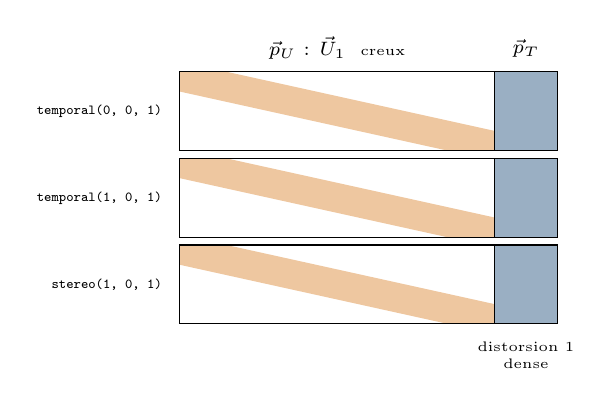
\begin{tikzpicture}[x=1cm, y=1cm]
        % blocs colonnes : U_1 (0..4), distorsion 1 (4..4.8)
        \foreach \r/\lab in {0/{\code{temporal(0, 0, 1)}}, 1/{\code{temporal(1, 0, 1)}}, 2/{\code{stereo(1, 0, 1)}}}{
          \pgfmathsetmacro{\yt}{-1.1*\r}
          \pgfmathsetmacro{\yb}{-1.1*\r-1.0}
          \fill[pyorange!45] (0,\yt) -- (0.6,\yt) -- (4,\yb+0.25) -- (4,\yb) -- (3.4,\yb) -- (0,\yt-0.25) -- cycle;
          \fill[pyblue!45] (4,\yt) rectangle (4.8,\yb);
          \draw (0,\yt) rectangle (4.8,\yb);
          \draw (4,\yt) -- (4,\yb);
          \node[font=\tiny, anchor=east] at (-0.1,\yt-0.5) {\lab};
        }
        \node[font=\scriptsize] at (2,0.3) {$\vec{p}_U$ : $\vec{U}_1$ \ \tiny creux};
        \node[font=\scriptsize] at (4.4,0.3) {$\vec{p}_T$};
        \node[font=\tiny, align=center] at (4.4,-3.6) {distorsion 1\\dense};
      \end{tikzpicture}
    \end{column}
    \begin{column}{0.46\textwidth}\footnotesize
      Pour chaque vue d'un appariement :
      \begin{itemize}
        \item \alert{déplacement} de sa frame (si optimisée) :
              \code{jacobian\_dx} $\times$ fonctions de forme : bloc
              \alert{creux} (sommets de l'élément du point) ;
        \item chaque \alert{transformation} optimisée de sa caméra :
              \code{jacobian\_d\{kind\}}, bloc \alert{dense} de $n_p$ colonnes ;
        \item $-$ vue 1, $+$ vue 2 ; transformation partagée ou même frame en
              stéréo : \alert{sommées} dans les mêmes colonnes ;
        \item structure creuse \alert{fixe} (calculée une fois, CSR triée) : un
              point hors de l'image donne des zéros explicites.
      \end{itemize}
    \end{column}
  \end{columns}
\end{frame}

% ---------------------------------------------------------------------
\begin{frame}[fragile]{Exemple complet : une mesure}
\begin{lstlisting}[basicstyle=\ttfamily\tiny]
import numpy, pysolvegn
from pysdic import (IntegrationPoints, Pairing, create_bicamera_analysis, SDICCorrelationTerm, SDICUnknowns,
                    compute_gray_level_groups, compute_visibility, display_residual_maps)
 
analysis = create_bicamera_analysis(mesh, left, right, left_images, right_images)
analysis.set_zero_displacement(0)
analysis.set_displacement(1, first_guess)
 
ip = IntegrationPoints.from_gauss_points("quadrangle_4", mesh.n_elements)
for view in analysis.get_views(1):                  # garde-fou : points vus ?
    print(compute_visibility(mesh, ip, view, warp_by=first_guess).mean())
 
pairings = [Pairing.temporal(0, 0, 1), Pairing.temporal(1, 0, 1), Pairing.stereo(1, 0, 1)]
groups = compute_gray_level_groups(analysis.mesh, ip, neighborhood=1)  # une fois
unknowns = SDICUnknowns([1], [])                    # U_1 inconnu, caméras fixes
correlation = SDICCorrelationTerm(analysis, unknowns, ip, pairings,
                                  gl_correction={"mode": "ZNSSD", "scale": 255.0},
                                  gray_level_groups=groups, use_cache=True)
 
result = pysolvegn.solve(terms=[correlation.term], p0=analysis.pack_unknowns(unknowns), max_iteration=30)
analysis.apply_unknowns(unknowns, result.parameters)  # U_1 écrit dans l'analyse
display_residual_maps(analysis, correlation.compute_residuals()[2])  # stéréo, ZNSSD
analysis.to_archive("mesure.zip", title="Mesure bicaméra")
\end{lstlisting}
\end{frame}

% ---------------------------------------------------------------------
\begin{frame}{Qui dépend de quoi}
  \centering
  \resizebox{!}{5.6cm}{%
  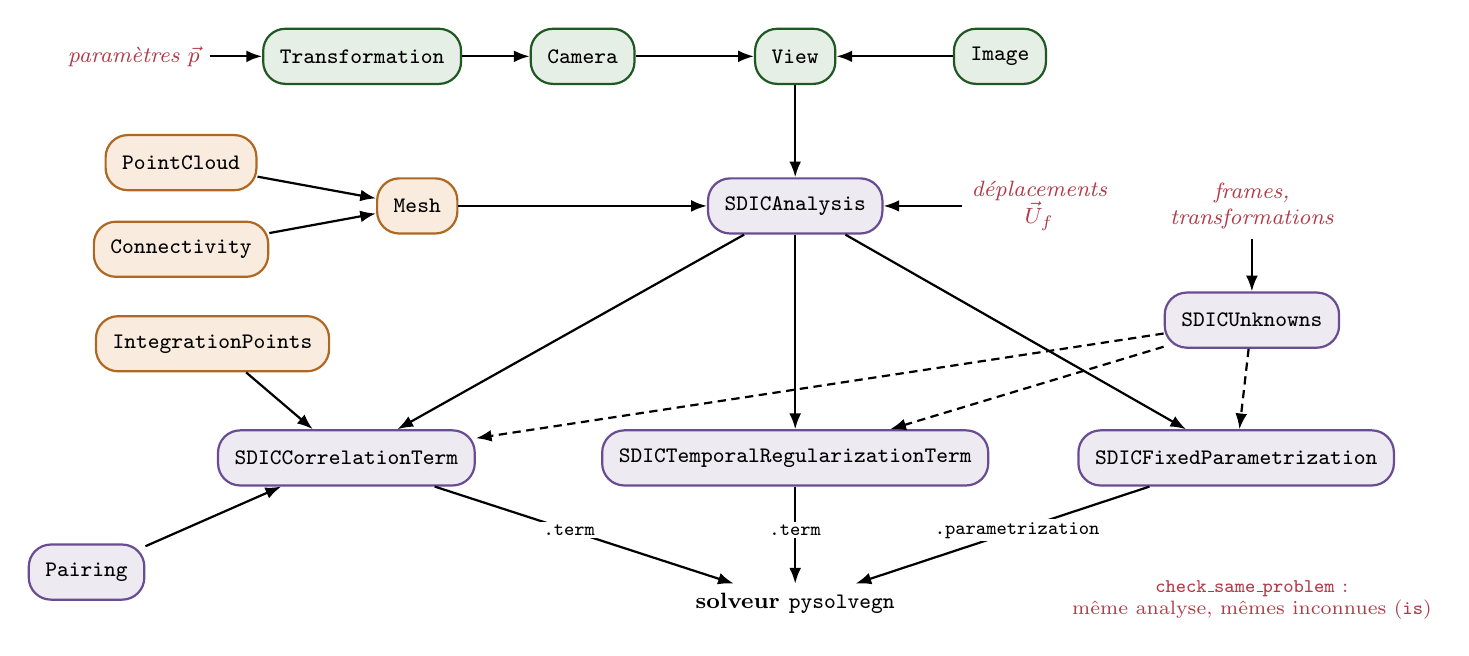
\begin{tikzpicture}[
      bubble/.style={draw, thick, rounded corners=8pt, minimum height=0.7cm, inner xsep=6pt, font=\footnotesize\ttfamily},
      geo/.style={bubble, fill=pyorange!15, draw=pyorange!80!black},
      img/.style={bubble, fill=pygreen!12, draw=pygreen!70!black},
      sdic/.style={bubble, fill=pypurple!12, draw=pypurple},
      state/.style={font=\footnotesize\itshape, text=pyred, align=center},
      dep/.style={->, thick, >={Latex[length=2mm]}},
      lab/.style={font=\scriptsize\ttfamily, fill=white, inner sep=1pt}]
    % Imagerie
    \node[state] (params) at (0,4.2) {paramètres $\vec{p}$};
    \node[img] (tr) at (2.9,4.2) {Transformation};
    \node[img] (cam) at (5.7,4.2) {Camera};
    \node[img] (view) at (8.4,4.2) {View};
    \node[img] (image) at (11.0,4.2) {Image};
    \draw[dep] (params) -- (tr);
    \draw[dep] (tr) -- (cam);
    \draw[dep] (cam) -- (view);
    \draw[dep] (image) -- (view);
    % Géométrie
    \node[geo] (pc) at (0.6,2.85) {PointCloud};
    \node[geo] (conn) at (0.6,1.75) {Connectivity};
    \node[geo] (mesh) at (3.6,2.3) {Mesh};
    \draw[dep] (pc) -- (mesh);
    \draw[dep] (conn) -- (mesh);
    % Analyse
    \node[sdic] (analysis) at (8.4,2.3) {SDICAnalysis};
    \node[state] (disp) at (11.5,2.3) {déplacements\\$\vec{U}_f$};
    \draw[dep] (view) -- (analysis);
    \draw[dep] (mesh) -- (analysis);
    \draw[dep] (disp) -- (analysis);
    \node[sdic] (unknowns) at (14.2,0.85) {SDICUnknowns};
    \node[state] (choice) at (14.2,2.3) {frames,\\transformations};
    \draw[dep] (choice) -- (unknowns);
    % Termes et paramétrisation
    \node[sdic] (corr) at (2.7,-0.9) {SDICCorrelationTerm};
    \node[sdic] (reg) at (8.4,-0.9) {SDICTemporalRegularizationTerm};
    \node[sdic] (fix) at (14.0,-0.9) {SDICFixedParametrization};
    \node[geo] (ip) at (1.0,0.55) {IntegrationPoints};
    \node[sdic] (pairing) at (-0.6,-2.35) {Pairing};
    \draw[dep] (analysis) -- (corr);
    \draw[dep] (analysis) -- (reg);
    \draw[dep] (analysis) -- (fix);
    \draw[dep, densely dashed] (unknowns) -- (corr);
    \draw[dep, densely dashed] (unknowns) -- (reg);
    \draw[dep, densely dashed] (unknowns) -- (fix);
    \draw[dep] (ip) -- (corr);
    \draw[dep] (pairing) -- (corr);
    % Solveur
    \node[font=\footnotesize\bfseries] (solver) at (8.4,-2.75) {solveur \texttt{pysolvegn}};
    \draw[dep] (corr) -- node[lab, pos=0.45] {.term} (solver);
    \draw[dep] (reg) -- node[lab, pos=0.45] {.term} (solver);
    \draw[dep] (fix) -- node[lab, pos=0.45] {.parametrization} (solver);
    \node[font=\scriptsize, text=pyred, align=center] at (14.2,-2.7)
      {\texttt{check\_same\_problem} :\\même analyse, mêmes inconnues (\texttt{is})};
  \end{tikzpicture}}

  \medskip
  \small
  $A \to B$ : $B$ \alert{utilise} $A$, sans copie : modifier \textcolor{pyred}{\textit{les
  paramètres}} ou \textcolor{pyred}{\textit{les déplacements}} agit sur tout ce qui est
  \alert{en aval}. Les bulles sont figées : on en crée une nouvelle (\texttt{with\_...}).
  \cls{SDICUnknowns} ne connaît pas l'analyse (pointillés) : l'analyse la valide.
\end{frame}

% =====================================================================
\section{Outils complémentaires}
% =====================================================================
 
% ---------------------------------------------------------------------
\begin{frame}[fragile]{Régularisation temporelle}
  \begin{columns}[T]
    \begin{column}{0.50\textwidth}\scriptsize
      \centering
      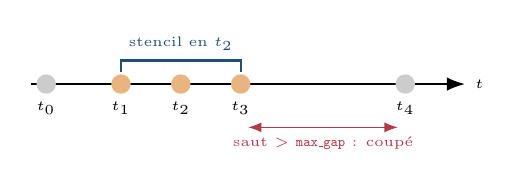
\begin{tikzpicture}[x=0.95cm]
        \draw[->,thick] (-0.2,0) -- (5.6,0) node[right,font=\tiny]{$t$};
        \foreach \t/\f/\c in {0/0/gray!40, 1/1/pyorange!60, 1.8/2/pyorange!60, 2.6/3/pyorange!60, 4.8/4/gray!40}{
          \fill[\c] (\t,0) circle (3.5pt);
          \node[font=\tiny, below=3pt] at (\t,0) {$t_\f$};
        }
        \draw[pyblue,thick] (1.0,0.15) -- (1.0,0.3) -- (2.6,0.3) -- (2.6,0.15);
        \node[font=\tiny, pyblue, above] at (1.8,0.3) {stencil en $t_2$};
        \draw[<->,pyred] (2.7,-0.55) -- (4.7,-0.55) node[midway,below,font=\tiny]{saut $>$ \texttt{max\_gap} : coupé};
      \end{tikzpicture}
 
      \raggedright\vspace{-2pt}
      \[
        r_{i,v,e} = \sqrt{w_e\,\omega_i}\,\Bigl(\textstyle\sum_k c_{i,k}\, u_{f_k,v,e}
        - a_{f_i,v,e}\Bigr)
      \]
      \begin{itemize}\setlength{\itemsep}{0pt}
        \item $c_{i,k}$ : différences finies d'ordre $n$ aux \alert{instants}
              \texttt{analysis.times} (obligatoires) ;
        \item \texttt{row\_weights="time"} : coût $\approx \int \|\vec{u}^{(n)} - \vec{a}\|^2\,dt$,
              indépendant de l'échantillonnage.
      \end{itemize}
    \end{column}
    \begin{column}{0.48\textwidth}
\begin{lstlisting}[basicstyle=\ttfamily\tiny]
from pysdic import (SDICTemporalRegularizationTerm,
                    check_same_problem)
 
analysis = create_bicamera_analysis(mesh, left, right,
    imgs_g, imgs_d, times=times)
unknowns = SDICUnknowns([1, 2, 3], [])
correlation = SDICCorrelationTerm(analysis, unknowns, ip, pairings)
reg = SDICTemporalRegularizationTerm(
    analysis, unknowns, order=2,
    accuracy=2,             # ordre des stencils
    boundary="one_sided",   # ou "valid"
    max_gap=None,           # coupe les grands sauts
    row_weights="time",     # ou "uniform"
    weight=1e-2)
 
check_same_problem([correlation, reg])
result = pysolvegn.solve([correlation.term, reg.term],
                         analysis.pack_unknowns(unknowns))
analysis.apply_unknowns(unknowns, result.parameters)
softer = reg.with_options(order=1, weight=1e-1)
\end{lstlisting}
      \tiny \alert{Mêmes objets} analyse et \cls{SDICUnknowns} que la corrélation
      (\texttt{check\_same\_problem}) : les termes s'additionnent. Nouvelles inconnues : \texttt{reg.with\_unknowns(unknowns)}.
      Aussi : \texttt{target}, \texttt{component\_weights}.
    \end{column}
  \end{columns}
\end{frame}

% ---------------------------------------------------------------------
\begin{frame}[fragile]{Choisir les inconnues : paramétrisation fixe}
  \begin{columns}[T]
    \begin{column}{0.47\textwidth}\scriptsize
      Les termes restent sur le vecteur \alert{complet} $\vec{p}$. Le solveur optimise
      $\vec{q}$, une sélection de $\vec{p}$ :
      \[
        \vec{p} = P(\vec{q}) = S\,\vec{q} + \vec{p}_{\text{fixe}},
        \qquad \mathbf{J}_q = \mathbf{J}_p\, S
      \]
      \begin{itemize}\setlength{\itemsep}{0pt}
        \item \texttt{vertices} et \texttt{components} choisis ; transformations
              optimisées : toutes ;
        \item \texttt{compute\_supported\_vertices} : sommets portant des points ;
        \item sur l'analyse et les \cls{SDICUnknowns} du problème ; \texttt{.parametrization}
              pour le solveur ;
        \item $\vec{p}_{\text{fixe}}$ relu \alert{à chaque appel} de \texttt{p\_func} :
              rien à reconstruire après une convergence ;
      \end{itemize}
      \textcolor{pyred}{Attention :} \texttt{pysolvegn.Parametrization}
      ($\vec{q} \mapsto \vec{p}$ du solveur) $\neq$ \cls{Parametrization}
      (paramètres d'une transformation).
    \end{column}
    \begin{column}{0.51\textwidth}
\begin{lstlisting}[basicstyle=\ttfamily\tiny]
# 1. Inconnues et termes sur le p complet
unknowns = SDICUnknowns(frames, [])
corr = SDICCorrelationTerm(analysis, unknowns, ip, pairings)
reg = SDICTemporalRegularizationTerm(
    analysis, unknowns, order=2, weight=1e-2)
# 2. Paramétrisation : même analyse, mêmes inconnues
vertices = compute_supported_vertices(analysis.mesh, ip)
param = SDICFixedParametrization(
    analysis, unknowns, vertices=vertices, components=[0, 1])
check_same_problem([corr, reg, param])
# 3. Résolution en q, retour à p
result = pysolvegn.solve([corr.term, reg.term],
    param.reparametrized_pack(),
    parametrization=param.parametrization)
param.reparametrized_apply(result.parameters)
\end{lstlisting}
      \vspace{-2pt}
      \fcolorbox{pyred}{pyred!8}{\parbox{0.95\linewidth}{\scriptsize\color{pyred}
        \textbf{Avec une paramétrisation, il FAUT utiliser}
        \texttt{param.reparametrized\_pack/unpack/apply} (vecteur réduit $\vec{q}$),
        \textbf{jamais} \texttt{analysis.*\_unknowns} (vecteur complet $\vec{p}$).}}
    \end{column}
  \end{columns}
\end{frame}

% ---------------------------------------------------------------------
\begin{frame}[fragile]{Corrections des niveaux de gris}
  \begin{columns}[T]
    \begin{column}{0.50\textwidth}\footnotesize
      \textbf{ZNSSD} (mode par défaut) : les deux vues normalisées
      \[
        g' = \text{scale}\cdot\frac{g - m}{s}
      \]
      \textbf{Matching} : la vue 2 ramenée sur la vue 1
      \[
        g_2' = \text{scale}\cdot\Bigl(\frac{(g_2 - m_2)\,s_1}{s_2} + m_1\Bigr)
      \]
      \textcolor{pyred}{Attention :} avec plusieurs appariements, ils n'ont plus le
      même poids.
 
      \smallskip
      Statistiques globales ou par \alert{voisinage} d'éléments (groupes qui se
      recouvrent). Points hors ROI ignorés. Les groupes ne dépendent que du maillage
      et des points : \texttt{compute\_gray\_level\_groups} \alert{une fois}, puis
      \texttt{gray\_level\_groups=groups} pour tous les termes.
    \end{column}
    \begin{column}{0.48\textwidth}
\begin{lstlisting}[basicstyle=\ttfamily\tiny]
gl_correction = {           # None : aucune
    "mode": "ZNSSD",       # "matching"
    "jacobian": "approximate",  # "exact"
    "neighborhood": None,  # ou n >= 0
    "scale": 255.0,        # défaut : 1.0
}
\end{lstlisting}
      \footnotesize
      \begin{itemize}
        \item \code{"approximate"} : $m$, $s$ constants,
              $\partial g' \approx \tfrac{\text{scale}}{s}\,\partial g$ ;
        \item \code{"exact"} : matrice creuse $D$ appliquée aux jacobiennes brutes,
              $\mathbf{J} = (D_{2\cdot} - D_{1\cdot})\,\mathbf{J}_{\text{brut}}$ ;
              dense pour un groupe global ;
        \item s'applique aussi aux colonnes des transformations ;
        \item fonctions séparées : \code{znssd\_correction(\_exact)},
              \code{matching\_correction(\_exact)}.
      \end{itemize}
    \end{column}
  \end{columns}
\end{frame}

% ---------------------------------------------------------------------
\begin{frame}[fragile]{Caches : explicites, jamais par défaut}
  \begin{columns}[T]
    \begin{column}{0.50\textwidth}\scriptsize
      \textbf{Terme de corrélation} \hfill \texttt{use\_cache=True}
      \begin{itemize}\setlength{\itemsep}{0pt}
        \item \alert{opérateurs} ($\vec{r}, \mathbf{J}$ ou $\vec{g}, \mathbf{H}, c$) rendus
              pour le même $\vec{p}$ \alert{si rien n'a bougé} ;
        \item \alert{vues de référence} projetées une fois, refaites si leur
              déplacement ou leur caméra change ;
        \item un nouveau terme (\texttt{with\_...}) part de caches vides.
      \end{itemize}
      \smallskip
      \textbf{Polynômes de Zernike} \hfill \cls{ZernikePolynomialsCache}
      \begin{itemize}\setlength{\itemsep}{0pt}
        \item les $Z_j(x, y)$ pour des points et une ellipse $(R_x, R_y, x_0, y_0)$ ;
        \item utile si les points normalisés ne bougent pas (étalonnage de la
              distorsion seule) ;
        \item \alert{partageable}, LRU (\texttt{max\_entries}).
      \end{itemize}
    \end{column}
    \begin{column}{0.48\textwidth}
\begin{lstlisting}[basicstyle=\ttfamily\tiny]
import pysdic
 
# Une distorsion partagée par les vues L et R
cache = pysdic.ZernikePolynomialsCache(max_entries=2)
distortion.polynomials_cache = cache
 
unknowns = pysdic.SDICUnknowns([], [("distortion", d)])
correlation = pysdic.SDICCorrelationTerm(
    analysis, unknowns, ip, [pysdic.Pairing.stereo(f, 0, 1)],
    sparse=False, use_cache=True)
result = pysolvegn.solve(terms=[correlation.term],
                         p0=analysis.pack_unknowns(unknowns))
analysis.apply_unknowns(unknowns, result.parameters)
 
print(cache)  # n_entries, nbytes, hits, misses
distortion.polynomials_cache = None   # retiré
cache.clear()                         # mémoire libérée
\end{lstlisting}
      \tiny \textcolor{pyred}{Attention :} environ $8\,N_p (2 + P)$ octets par entrée
      ($P$ polynômes) ; inutile en mesure (les points bougent).
    \end{column}
  \end{columns}
\end{frame}

% ---------------------------------------------------------------------
\begin{frame}[fragile]{Diagnostic : les résidus}
  \begin{columns}[T]
    \begin{column}{0.57\textwidth}
\begin{lstlisting}[basicstyle=\ttfamily\tiny]
from pysdic import (Pairing, compute_residuals,
    compute_pixel_residual_maps, display_residual_maps)

# Aux points d'intégration : un PairingResiduals
pairing = Pairing.stereo(1, 0, 1)
gl = {"mode": "ZNSSD", "scale": 255.0}
res = compute_residuals(analysis, pairing, ip, gl_correction=gl)
res.gray_levels_1, res.gray_levels_2   # (N_p, C)
res.residuals                          # g'_2 - g'_1

# Au pixel, tracé dans les deux vues
map_1, map_2 = compute_pixel_residual_maps(analysis, res,
                                           fill_radius=1.0)
display_residual_maps(analysis, res)

# Ce que compare un terme, pour un vecteur p
residuals = correlation.compute_residuals(p)  # un par appariement

# Contrôle qualité : RMS par élément, éléments suspects
from pysdic.workflows import compute_elements_residual_rms
quality = compute_elements_residual_rms(analysis, ip, residuals)
quality.bad_elements
\end{lstlisting}
    \end{column}
    \begin{column}{0.40\textwidth}\footnotesize
      \begin{itemize}\setlength{\itemsep}{2pt}
        \item les niveaux de gris des deux vues d'un appariement et leur différence,
              avec la \alert{même} correction que le terme, sans les poids ;
        \item le résidu appartient au point matériel : tracé à sa projection
              dans \alert{chaque} vue ;
        \item la carte au pixel montre \alert{où} la corrélation est mauvaise
              (reflets, zones cachées\dots) ;
        \item \texttt{pysdic.workflows} : RMS par élément et par appariement,
              incertitude des déplacements.
      \end{itemize}
    \end{column}
  \end{columns}
\end{frame}

% ---------------------------------------------------------------------
\begin{frame}[fragile]{Images synthétiques}
  \begin{columns}[T]
    \begin{column}{0.49\textwidth}
      \textbf{Lancer de rayons} \hfill \small vérité exacte
\begin{lstlisting}[basicstyle=\ttfamily\tiny]
from pysdic import (compute_wave_speckle,
    generate_synthetic_image, add_gaussian_noise,
    quantize_image)

texture = compute_wave_speckle(uv_points, wavelength=0.15)
image = generate_synthetic_image(camera, mesh, texture,
    displacement=U, n_samples=3)        # (H, W, 1)
image = quantize_image(add_gaussian_noise(image, std=1.0),
                       bit_depth=8)
\end{lstlisting}
      \scriptsize
      \begin{itemize}\setlength{\itemsep}{0pt}
        \item un rayon par sous-pixel, intersecté avec le maillage déformé ;
        \item la texture suit le \alert{point matériel} (UV map) : niveaux de gris
              conservés, sans éclairage ;
        \item bruit, flou, quantification : fonctions séparées.
      \end{itemize}
    \end{column}
    \begin{column}{0.49\textwidth}
      \textbf{Blender} \hfill \small \texttt{pysdic-blender}
\begin{lstlisting}[basicstyle=\ttfamily\tiny]
from pysdic_blender import (BlenderCamera, BlenderMesh,
    BlenderExperiment, BlenderSpotLight, get_steel_material)

experiment = BlenderExperiment(background_strength=0.1)
experiment.add_camera("left", BlenderCamera(camera))
experiment.add_spotlight("spot", BlenderSpotLight.looking_at(
    [300, 0, 600], [0, 0, 0], energy=5e5))
experiment.add_mesh("plate", BlenderMesh(mesh, texture=texture),
                    material=get_steel_material())
intensity = experiment.render("left", n_samples=128)
\end{lstlisting}
      \scriptsize
      \begin{itemize}\setlength{\itemsep}{0pt}
        \item Cycles : ombres, reflets, matériaux (Principled BSDF) ;
        \item caméra OpenCV sténopé \alert{vérifiée}, maillage \code{triangle\_3} ;
        \item package \alert{séparé} : \texttt{bpy} impose la version de Python de Blender (3.13).
      \end{itemize}
    \end{column}
  \end{columns}
\end{frame}

% ---------------------------------------------------------------------
\begin{frame}[plain]{}
  \centering
  
\begin{tikzpicture}[line join=round, line cap=round]
    \definecolor{foxorange}{HTML}{E07A2E}
    \definecolor{foxdark}{HTML}{3B2A20}
    % Queue
    \fill[foxorange] (1.15,-1.55) .. controls (2.6,-1.9) and (3.3,-0.6) .. (2.75,0.35)
      .. controls (2.45,-0.45) and (1.95,-0.95) .. (1.2,-1.05) -- cycle;
    \begin{scope}
      \clip (1.15,-1.55) .. controls (2.6,-1.9) and (3.3,-0.6) .. (2.75,0.35)
        .. controls (2.45,-0.45) and (1.95,-0.95) .. (1.2,-1.05) -- cycle;
      \fill[white] (2.85,0.25) circle (0.5);
    \end{scope}
    % Corps
    \fill[foxorange] (-1.05,-1.95) .. controls (-1.3,-0.9) and (-0.85,-0.35) .. (0,-0.3)
      .. controls (0.85,-0.35) and (1.3,-0.9) .. (1.05,-1.95) -- cycle;
    \fill[white] (-0.42,-1.95) .. controls (-0.5,-1.1) and (-0.3,-0.65) .. (0,-0.6)
      .. controls (0.3,-0.65) and (0.5,-1.1) .. (0.42,-1.95) -- cycle;
    % Pattes
    \fill[foxdark] (-0.75,-2.1) rectangle (-0.4,-1.85);
    \fill[foxdark] (0.4,-2.1) rectangle (0.75,-1.85);
    % Oreilles
    \fill[foxorange] (-1.0,0.75) -- (-0.75,1.85) -- (-0.15,0.95) -- cycle;
    \fill[foxorange] (1.0,0.75) -- (0.75,1.85) -- (0.15,0.95) -- cycle;
    \fill[foxdark] (-0.82,1.0) -- (-0.72,1.55) -- (-0.4,1.05) -- cycle;
    \fill[foxdark] (0.82,1.0) -- (0.72,1.55) -- (0.4,1.05) -- cycle;
    % Tête
    \fill[foxorange] (-1.25,0.85) .. controls (-1.2,0.2) and (-0.6,-0.45) .. (0,-0.75)
      .. controls (0.6,-0.45) and (1.2,0.2) .. (1.25,0.85)
      .. controls (0.7,1.15) and (-0.7,1.15) .. cycle;
    \fill[white] (-1.2,0.6) .. controls (-0.85,0.05) and (-0.35,-0.35) .. (0,-0.75)
      .. controls (-0.1,-0.25) and (-0.3,0.15) .. (-0.6,0.3) .. controls (-0.85,0.45) .. cycle;
    \fill[white] (1.2,0.6) .. controls (0.85,0.05) and (0.35,-0.35) .. (0,-0.75)
      .. controls (0.1,-0.25) and (0.3,0.15) .. (0.6,0.3) .. controls (0.85,0.45) .. cycle;
    % Yeux et truffe
    \fill[foxdark] (-0.42,0.38) ellipse (0.09 and 0.13);
    \fill[foxdark] (0.42,0.38) ellipse (0.09 and 0.13);
    \fill[white] (-0.39,0.43) circle (0.03);
    \fill[white] (0.45,0.43) circle (0.03);
    \fill[foxdark] (0,-0.62) ellipse (0.13 and 0.09);
    % Texte
    \node[font=\Huge\bfseries, text=pyblue] at (5.6,0.35) {Merci !};
    \node[font=\small, text=gray] at (5.6,-0.55) {Questions\,?};
  \end{tikzpicture}
\end{frame}

% ---------------------------------------------------------------------
\begin{frame}{Références}
  \small
  \begin{itemize}
    \item H.~Matar. \emph{Développement d'un outil de corrélation d'images stéréo :
          formulation d'un potentiel unique.} Thèse de doctorat, Matériaux,
          Université Clermont Auvergne, 2025. NNT : 2025UCFA0186.
          HAL : tel-05612939. \hfill (\alert{uCheckmate})
    \item Modèles de caméra et de distorsion : documentation OpenCV
          \texttt{calib3d}.
    \item \texttt{pysolvegn} : solveur de moindres carrés de Gauss--Newton (termes
          \code{rJ} / \code{gH}).
  \end{itemize}
\end{frame}
 
\end{document}